\chapterhead{System Design}

\sectionhead{System Overview}

The system has three parts: a reader at the door, a reader at the cabinet, and
one server. Each reader is an ESP32 chip with a fingerprint sensor, a small
screen, and an electric lock.

The readers never decide anything by themselves. When someone scans a finger,
the sensor finds a match and gives back a slot number. The reader sends that
number to the server. The server decides, saves the result, and sends back a
yes or no.

This matters because a reader hangs on a wall where anyone can reach it. If a
reader could decide on its own, someone could open it and fool it. The server
sits in a locked place, so the decision stays safe.

Access happens in two steps. A finger at the door unlocks the door and starts a
120-second session for that one person. A finger at the cabinet opens it only if
it belongs to the same person, and only while the session is still running. A
registered finger with no session is refused, and the refusal is saved. This is
the double check that \textcite{mohammed2025} found cuts fake entries.

The 120-second figure is not arbitrary. \textcite{owasp2026} recommend an idle
timeout of 2 to 5 minutes for high-value applications, against 15 to 30 minutes
for low-risk ones, and a stockroom of shared equipment belongs in the first
group. We took the strictest end of that range. Two minutes is long enough to
cross a room and reach the cabinet, and short enough that a person who walks
away leaves nothing useful behind them.

When the cabinet opens, it shows a one-time code on its screen. The website will
not accept a borrow record without that code. So every written record matches a
real opening. Reader records can never be edited or deleted. This is the
protection \textcite{koisser2023} say a log needs.

\sectionhead{System Architecture}

The architecture is described at five levels. The first covers how the separate parts connect to one another. The four that follow look inside a single reader, at its processor, its memory, the pins it uses to reach the outside world, and the network it speaks over.

\subsectionhead{Overall System Architecture}

The system is three programs working together. The ESP32 firmware runs on the
two readers and handles the sensor, the screen, and the lock. The backend is a
server written in Rust that holds the database and makes every decision. The
frontend is a website, built with SvelteKit, where people sign in, enter what
they borrowed, and read the record. The readers talk only to the backend, never
to each other and never to the website.

Figure~\ref{fig:overall} follows one complete use through all three, with one
lane for each program. Solid arrows are requests and replies. Dashed arrows are
things that happen without anybody asking: the live feed updating on the
dashboard, and the person carrying the code from the cabinet screen to the
website. Every decision diamond sits in the backend lane, because the readers
only report what they read and act on the answer.

\begin{figure}[H]
\centering
\caption{One complete use, followed through the readers, the backend, and the
frontend}
\label{fig:overall}
\begin{tikzpicture}[flow, x=1mm, y=1mm,
  side/.style = {deny, text width=16mm, minimum width=18mm},
  end/.style = {term, minimum width=14mm}]

\draw[gray!55, dashed, rounded corners=3pt] (-19,8) rectangle (19,-172);
\draw[gray!55, dashed, rounded corners=3pt] (23,8) rectangle (84,-172);
\draw[gray!55, dashed, rounded corners=3pt] (87,8) rectangle (119,-172);
\node[lanetitle] at (0,9)    {ESP32 readers};
\node[lanetitle] at (53.5,9) {Backend server};
\node[lanetitle] at (103,9)  {Frontend website};

\node[term] (s1) at (0,0)    {Start};
\node[io]   (e1) at (0,-15)  {Read finger, send\\door:slot};
\node[proc] (b1) at (40,-15) {Check reader\\ID and secret};
\node[dec]  (b2) at (40,-32) {Reader and\\finger valid?};
\node[side] (r1) at (70,-32) {Refuse,\\reply deny};
\node[end]  (x1) at (70,-44) {Stop};
\node[proc] (b3) at (40,-54) {Open 120~s session,\\save door grant};
\node[proc] (e2) at (0,-54)  {Show Welcome,\\release door};
\node[io]   (f1) at (103,-54) {Live feed on\\dashboard};

\node[proc] (s2) at (0,-69)  {Walk to\\the cabinet};
\node[io]   (e3) at (0,-84)  {Read finger, send\\cabinet:slot};
\node[dec]  (b4) at (40,-84) {Live session\\for this user?};
\node[side] (r2) at (70,-84) {Save refusal,\\reply deny};
\node[end]  (x2) at (70,-97) {Stop};
\node[proc] (b5) at (40,-104) {Issue one-time code,\\save cabinet grant,\\queue SMS};
\node[proc] (e4) at (0,-104) {Release lock 4~s,\\show the code};

\node[io]   (f2) at (103,-120) {Type code and\\borrowed items};
\node[dec]  (b6) at (40,-136) {Code valid\\for this user?};
\node[side] (r3) at (70,-136) {Log rejected\\code, show error};
\node[end]  (x3) at (70,-149) {Stop};
\node[proc] (b7) at (40,-156) {Save checkout,\\mark code spent};
\node[proc] (f3) at (103,-156) {Checkout\\on record};
\node[end]  (x4) at (103,-167) {Stop};

\draw[arr] (s1.south) -- (e1.north);
\draw[arr] (e1.east) -- (b1.west);
\draw[arr] (b1.south) -- (b2.north);
\draw[arr] (b2.east) -- node[lbl, above] {no} (r1.west);
\draw[arr] (r1.south) -- (x1.north);
\draw[arr] (b2.south) -- node[lbl, right] {yes} (b3.north);
\draw[arr] (b3.west) -- node[lbl, above] {unlock} (e2.east);
\draw[dashedarr] (b3.east) -- (f1.west);
\draw[arr] (e2.south) -- (s2.north);
\draw[arr] (s2.south) -- (e3.north);
\draw[arr] (e3.east) -- (b4.west);
\draw[arr] (b4.east) -- node[lbl, above] {no} (r2.west);
\draw[arr] (r2.south) -- (x2.north);
\draw[arr] (b4.south) -- node[lbl, right] {yes} (b5.north);
\draw[arr] (b5.west) -- node[lbl, above] {code} (e4.east);
\draw[dashedarr] (b5.east) -| (f1.south);
\draw[dashedarr] (e4.south) |- node[lbl, above, pos=0.75] {person reads the code} (f2.west);
\draw[arr] (f2.south) |- ($(b6.north)+(0,5)$) -- (b6.north);
\draw[arr] (b6.east) -- node[lbl, above] {no} (r3.west);
\draw[arr] (r3.south) -- (x3.north);
\draw[arr] (b6.south) -- node[lbl, right] {yes} (b7.north);
\draw[arr] (b7.east) -- (f3.west);
\draw[arr] (f3.south) -- (x4.north);

\end{tikzpicture}

\end{figure}

If the door reader is out of Wi-Fi range, the cabinet reader can share its own
connection with it. This bridge is built into the cabinet firmware but is
switched off by default, since it is only needed where the door is too far from
the router.

\subsectionhead{Microcontroller Architecture}

Both readers use the ESP32. The chip carries two processors, each able to run at
up to 240 MHz, and is rated at 1079.96 CoreMark in that configuration
\parencite{espressif2025}. \textcite{rahman2026} reviewed the platform and
identified the combination of dual-core processing, integrated radios and
peripheral support as its principal strength, while naming limited on-chip
memory and real-time constraints as its standing weaknesses.

The second processor is what makes the workload here practical. The fingerprint
sensor is slow relative to the processor, so one core can wait on the sensor
while the other holds the network connection open.

\subsectionhead{Memory Architecture}

The chip provides 448 KB of ROM for start-up code, 520 KB of on-chip RAM for
running programs, and two smaller low-power regions of 8 KB each, with the
application image held in external flash and executed through a cache
\parencite{espressif2025}. Limited on-chip memory is the constraint
\textcite{rahman2026} single out as the platform's most persistent difficulty.

Table~\ref{tab:memory} shows how this project uses those regions. Our program
fills about 81 percent of the 1.2 MB partition set aside for it, which leaves
room to grow but not a great deal of it.

One design choice removes the memory pressure that \textcite{rahman2026}
describe. Fingerprints are never stored on our chip; they stay inside the
sensor, which returns only a slot number. Fingerprint data is the largest
structure the reader would otherwise hold, so leaving it on the sensor keeps the
520 KB of RAM \parencite{espressif2025} comfortable rather than tight.

\begin{table}[H]
\centering
\caption{How the chip uses its memory}
\label{tab:memory}
\begin{tabular}{@{}llp{58mm}@{}}
\toprule
Storage & Size & What we use it for \\
\midrule
ROM    & 448~KB & Start-up code. We do not change it. \\
RAM    & 520~KB & The running program and its working data. \\
Flash  & 1.2~MB & Our program. About 81\% full. \\
Sensor & Inside sensor & Fingerprints. Our chip never reads them. \\
\bottomrule
\end{tabular}
\end{table}

\subsectionhead{Input and Output Architecture}

The chip exposes 34 programmable pins, three serial ports capable of up to
5 MBaud, two I2C interfaces and four SPI controllers \parencite{espressif2025}.
Sigurado uses three of those classes and leaves SPI unused.

Table~\ref{tab:io} lists what we connected where. The fingerprint sensor is
given its own serial port because it exchanges packet messages continuously. The
screen uses I2C, which carries a display on two wires
\parencite{espressif2025}. The lock, button, and light need only single pins.

\begin{table}[H]
\centering
\caption{What is connected to which pin}
\label{tab:io}
\begin{tabular}{@{}lllc c@{}}
\toprule
Part & Connection & Door & Cabinet \\
\midrule
Fingerprint sensor & Serial port 2 & 16, 17 & 16, 17 \\
Screen             & I2C           & 21, 22 & 21, 22 \\
Sign-up button     & Pin (in)      & 4      & 4 \\
Status light       & Pin (out)     & 2      & 2 \\
Lock switch        & Pin (out)     & 5      & 5 \\
Door closed sensor & Pin (in)      & ---    & 18 \\
Buzzer             & Pin (out)     & ---    & 19 \\
Text message unit  & Serial port 1 & ---    & 26, 27, 25 \\
\bottomrule
\end{tabular}
\end{table}

The lock pin is the only one that moves something physical. The lock runs on its
own 12~V power, not from the chip. A relay acts as the switch between them. The
door lock stays open for 3 seconds and the cabinet lock for 4. The cabinet also has a small switch that tells us
whether the door really closed.

\subsectionhead{Communication Architecture}

Each reader joins the school Wi-Fi and sends messages to the server. Each reader
has its own ID and password. It does not use a person's login.

This matters. If someone steals a reader and opens it, they only get that
reader's password. They cannot pretend to be a person, and we can change that
one password without touching the other reader. \textcite{rahman2026} name
security setup as a common weak spot on this chip, and this is what it looks
like in practice.

Each reader also says ``I am still here'' every 30 seconds. That is how the
website shows which readers are working. All clocks are set from the internet,
so every record has a matching time.

\sectionhead{Block Diagram}

Figure~\ref{fig:block} shows the two physical units the system is built from.
On the left is the materials cabinet, with its reader set into the panel above
the bins. On the right is the door kiosk, a stand that holds the door reader at
hand height beside the entrance. Each is drawn next to the lumber frame it is
built on, so the finished unit and its skeleton can be compared directly.

\begin{figure}[H]
\centering
\caption{The cabinet and the door kiosk, each beside the frame it is built on}
\label{fig:block}
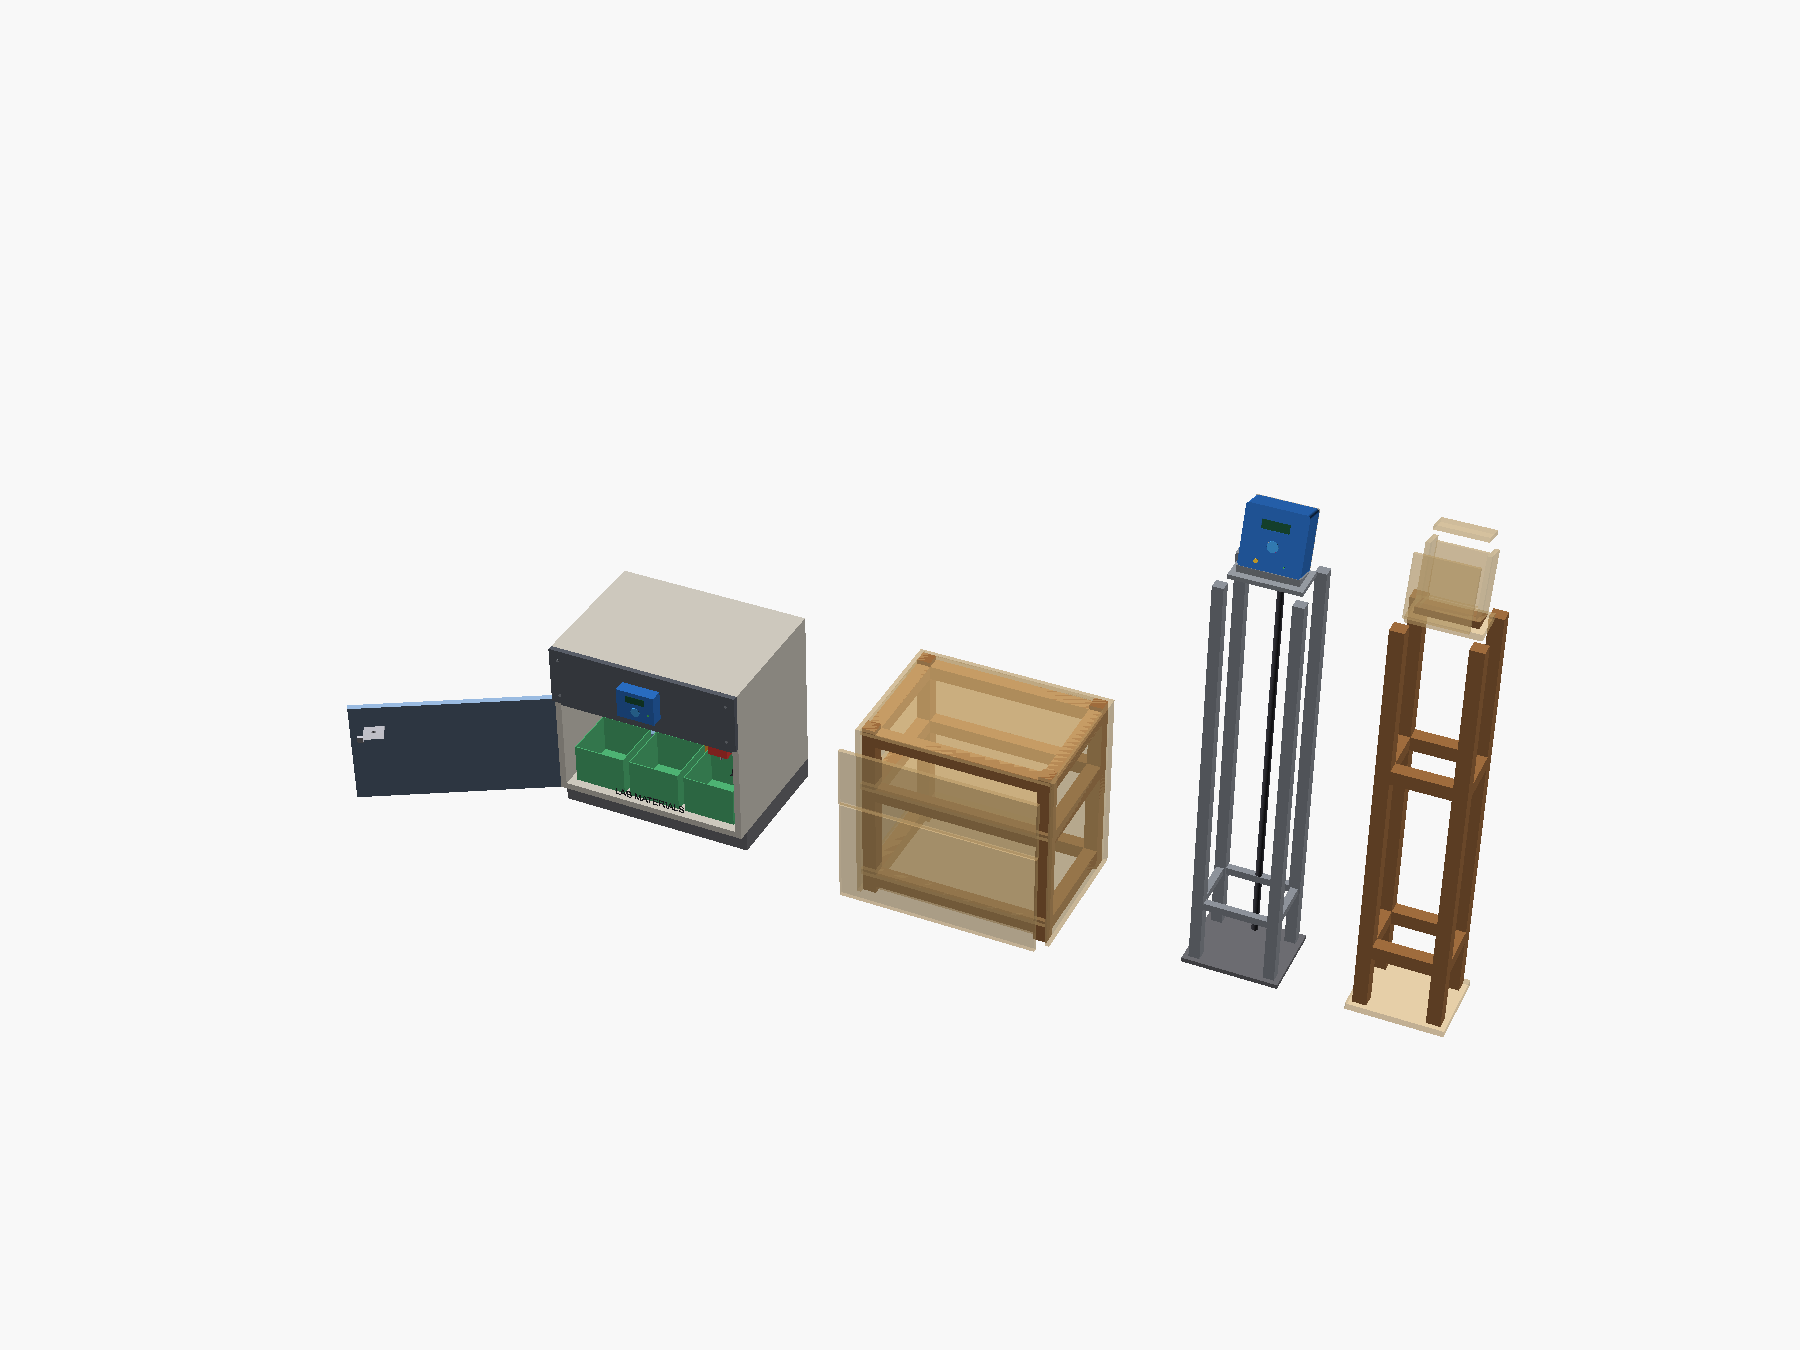
\includegraphics[width=\linewidth, trim=330 290 270 455, clip]{figures/all.png}
\end{figure}

\sectionhead{Hardware Components}

Table~\ref{tab:bom} lists every part used and the job it does. Quantities are per reader unless the entry says otherwise. Nothing on the list is rare or difficult to source, which was deliberate. A part that cannot be replaced from a local shop is a part that ends the project on the day it fails.

\begin{table}[H]
\centering
\caption{Parts used and what each one does}
\label{tab:bom}
\begin{tabular}{@{}p{32mm}p{78mm}@{}}
\toprule
Part & What it does \\
\midrule
ESP32 board &
  The small computer. Runs the program and connects to Wi-Fi. One per reader. \\
Fingerprint sensor (R307 or AS608) &
  Reads a finger and checks it against its own stored list. Fingerprints never
  leave it. \\
Small screen (16 by 2) &
  Shows messages. On the cabinet it also shows the one-time code. \\
Relay and 12~V lock &
  The relay is a switch. The lock runs on its own power, not the chip's. \\
Door switch &
  Cabinet only. Tells us if the door really closed. \\
SIM800L text unit &
  Cabinet only. Sends a text when the cabinet opens or someone is refused. \\
Buzzer, light, button &
  The button starts sign-up. The buzzer warns if the door is left open. \\
\bottomrule
\end{tabular}
\end{table}

\sectionhead{Hardware Architecture Design}

The cabinet and the reader box were drawn as 3D models before building. The
cabinet has three shelves behind locked doors. All the electronics sit in a
hidden space behind a screwed panel, so users never see them.

\begin{figure}[H]
\centering
\caption{The cabinet with its service panel removed, showing the electronics bay
above the materials bins}
\label{fig:3d}
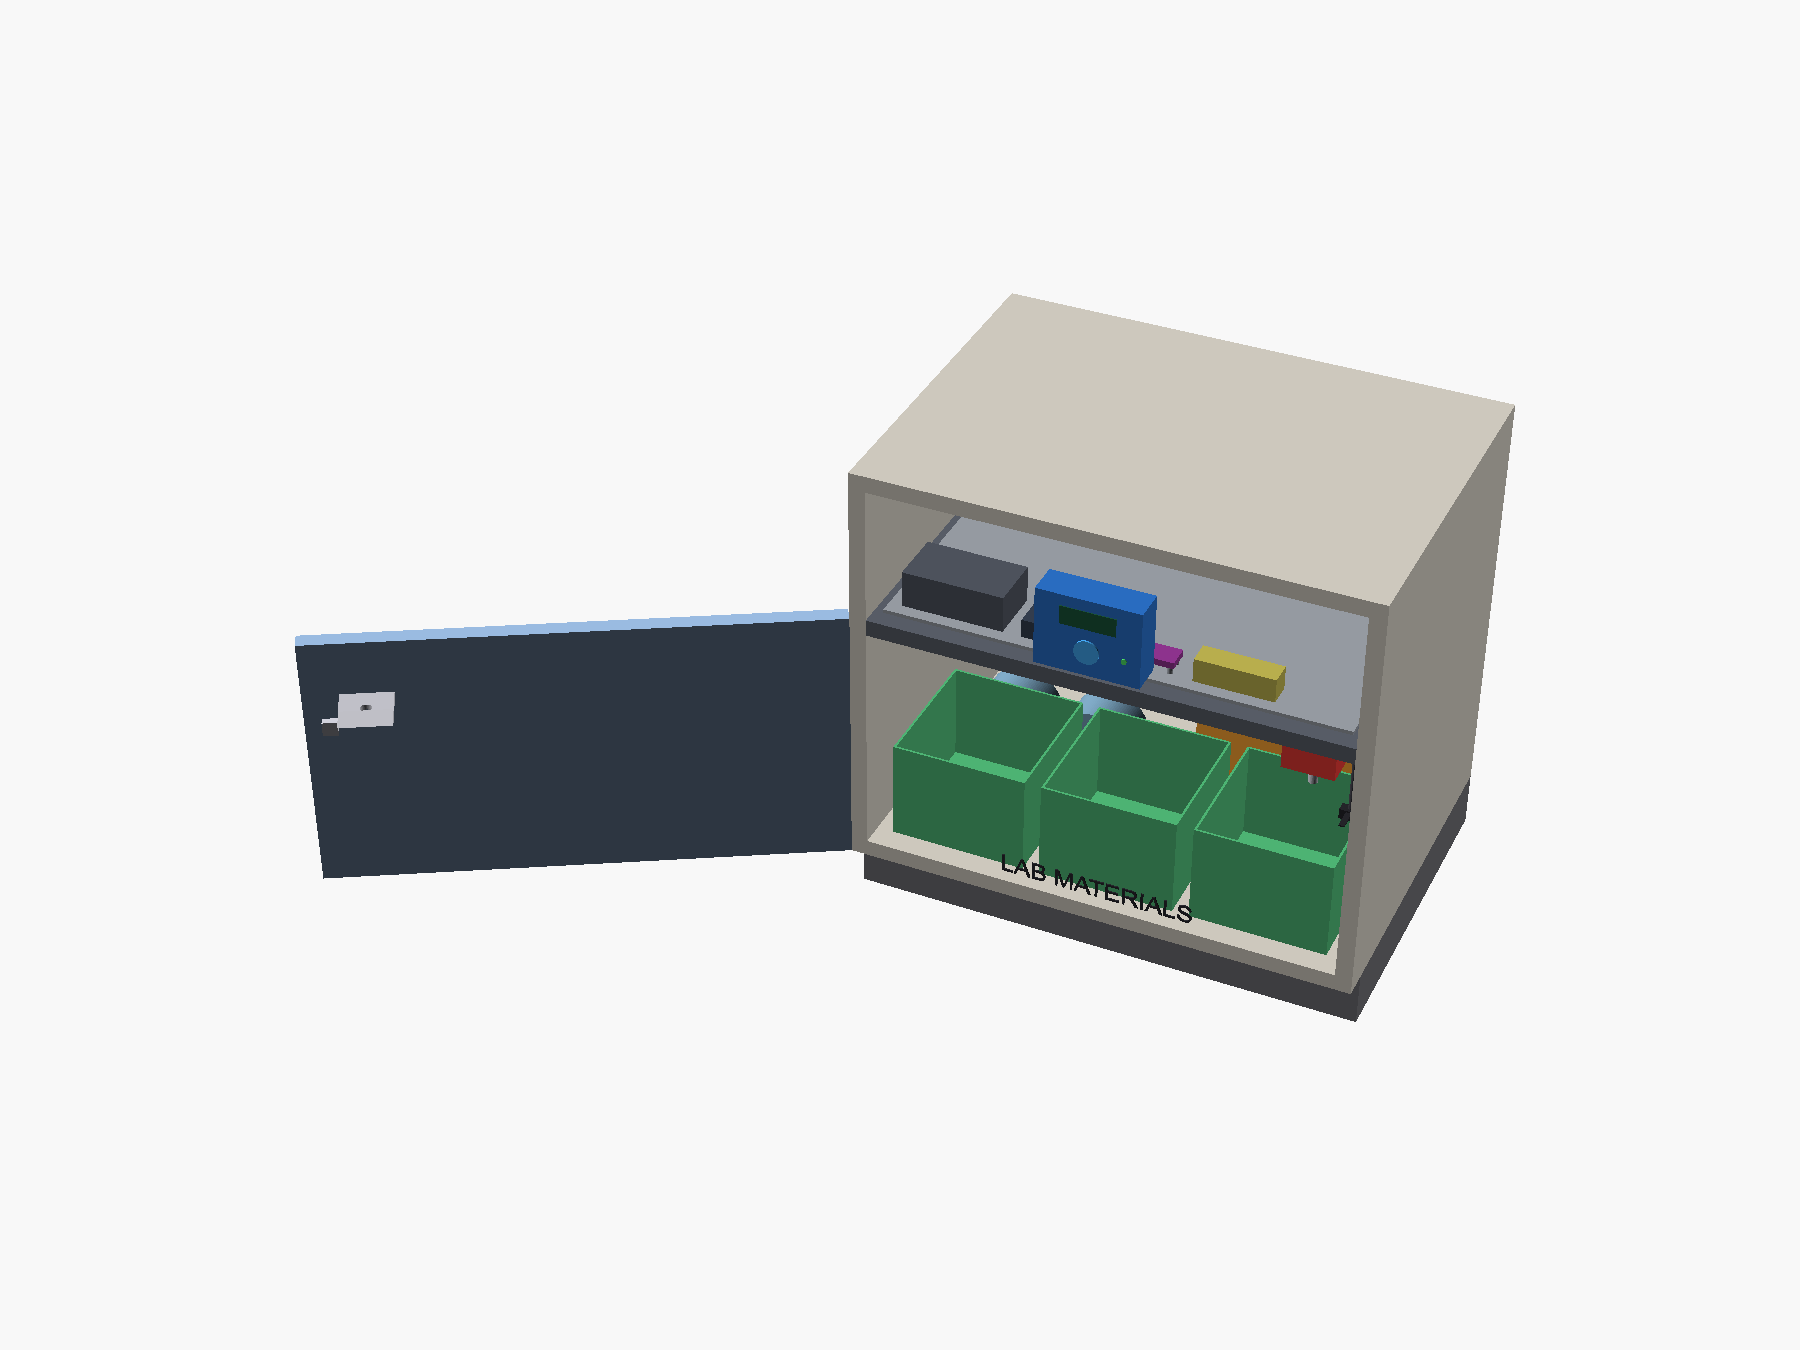
\includegraphics[width=0.92\linewidth]{figures/cabinet_service.png}
\end{figure}

Figure~\ref{fig:head} looks inside the reader box itself, with the back plate
taken off. This is the view used to check that every part fits and to plan the
wiring before anything was cut.

\begin{figure}[H]
\centering
\caption{Inside the reader box with the back plate removed, showing the board,
sensor, relay and lock wiring}
\label{fig:head}
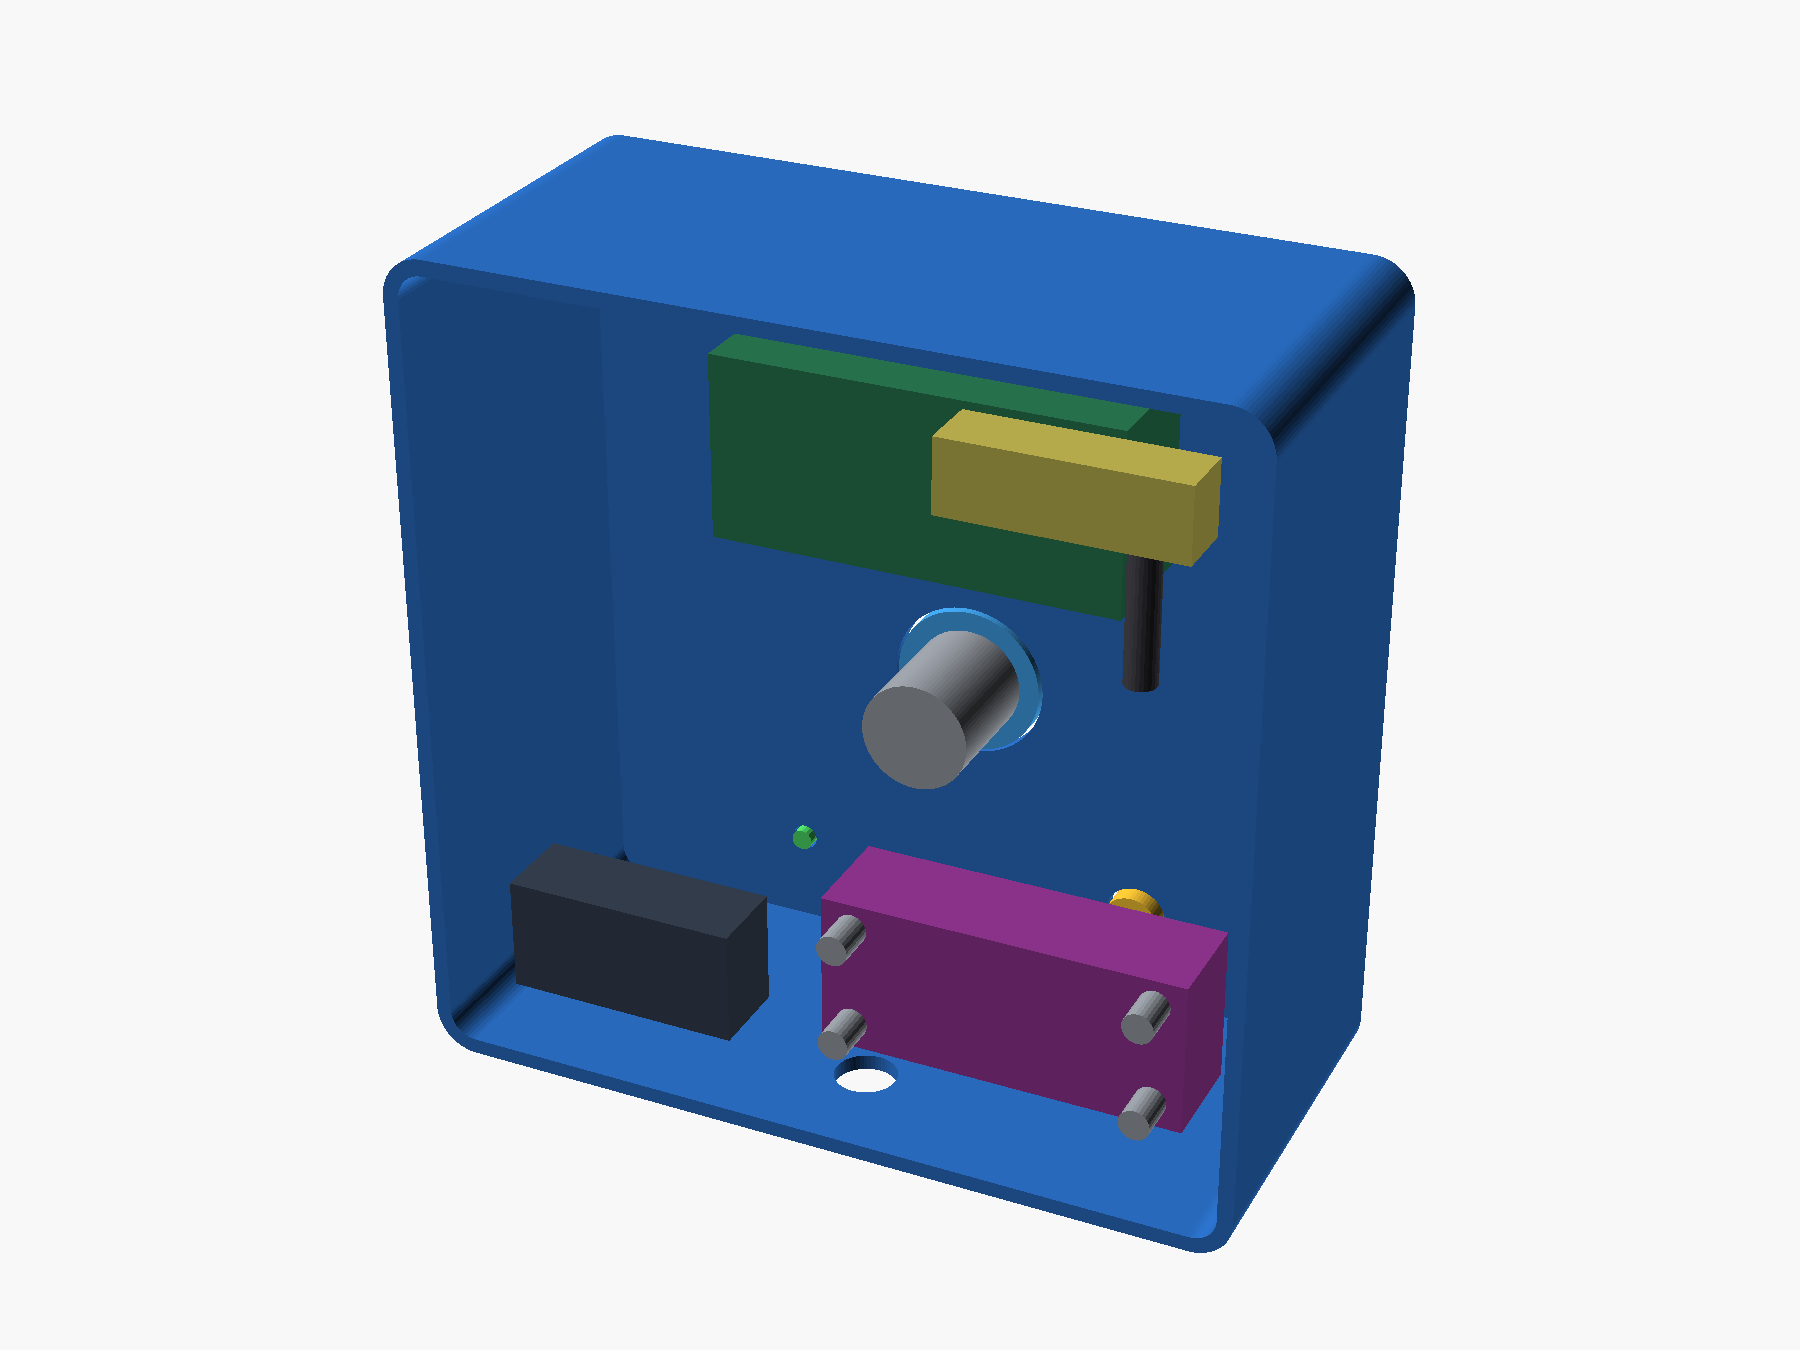
\includegraphics[width=0.82\linewidth]{figures/head_open.png}
\end{figure}

Wiring follows Table~\ref{tab:io}. Three rules guide the layout. First, the lock
gets its own power supply, because it pulls a lot of current when it opens and
would otherwise restart the chip. Second, the text unit also gets its own
supply, for the same reason. Third, one wire on the text unit needs a voltage
reducer, because the chip's signal is too strong for it.

\sectionhead{Data Flow}

Data passes through three programs on its way from a finger to the record: the
firmware on the ESP32 readers, the backend server, and the frontend website.
This section first lists the steps of one complete use, then follows the data
through each program in turn, with a flowchart for each. It ends one level
lower, with the instructions the chip itself executes.

\subsectionhead{Steps in One Complete Use}

The sequence below traces one successful use from beginning to end, from the
first finger at the door to the borrowed items appearing in the record. It is
the same path drawn in Figure~\ref{fig:overall}.

\begin{enumerate}
  \item Someone puts a finger on the door sensor. The sensor finds a match and
        gives back a slot number.
  \item The door reader sends that number, plus its own ID and password, to the
        server.
  \item The server looks up the person, starts a 120-second session, saves the
        record, and replies ``allowed''.
  \item The door reader opens the lock for 3 seconds and shows a message.
  \item Someone puts a finger on the cabinet sensor. The cabinet reader sends
        its own request.
  \item The server checks whether this is the same person who has the running
        session. If yes, it makes a one-time code and saves the record. If no,
        it refuses and saves that too.
  \item The cabinet releases its lock for 4 seconds and shows the code. The
        server queues a text message, which the cabinet sends on its next check.
        If the door is left open, the buzzer sounds.
  \item The person types the code and the borrowed items into the website. The
        server accepts it only if the code is still valid.
\end{enumerate}

\subsectionhead{The ESP32 Firmware}

Each reader runs one program that starts once and then repeats a single loop for
as long as it has power. Figure~\ref{fig:firmware} shows the cabinet reader,
which has the most to do. The door reader runs the same loop without the door
switch and the text messages. The only way out of the program is at start-up:
a reader whose fingerprint sensor does not answer shows an error and stops
there, since it has no work to do without one.

\begin{figure}[H]
\centering
\caption{The cabinet reader's firmware: start-up, then one pass of the loop}
\label{fig:firmware}
\begin{tikzpicture}[flow, x=1mm, y=0.93mm,
  proc/.append style={text width=24mm, minimum width=26mm},
  io/.append style={text width=19mm},
  end/.style = {term, minimum width=14mm}]

\node[term] (on)   at (0,0)    {Start};
\node[proc] (su1)  at (0,-12)  {Start serial, screen\\and lock};
\node[dec]  (sen)  at (0,-27)  {Sensor\\found?};
\node[deny] (hlt)  at (34,-27) {Show error\\and halt};
\node[end]  (x1)   at (62,-27) {Stop};
\node[proc] (su2)  at (0,-43)  {Join Wi-Fi, set clock,\\start SIM800L};
\node[proc] (mem)  at (0,-57)  {Check free memory};
\node[dec]  (door) at (0,-72)  {Door switch\\changed?};
\node[proc] (buzz) at (34,-72) {Warn at 30~s,\\alarm at 60~s};
\node[dec]  (btn)  at (0,-90)  {Enroll button\\pressed?};
\node[proc] (enr)  at (34,-90) {Run one\\enrollment step};
\node[io]   (poll) at (0,-106) {Poll sensor\\on UART2};
\node[dec]  (fp)   at (0,-121) {Finger\\matched?};
\node[io]   (scan) at (34,-121) {Send\\cabinet:slot};
\node[dec]  (ok)   at (68,-121) {Reply is\\unlock?};
\node[proc] (open) at (102,-137) {Release lock 4~s,\\show code 15~s};
\node[deny] (why)  at (68,-137) {Show the reason,\\stay locked};
\node[dec]  (hb)   at (0,-155) {30~s since\\heartbeat?};
\node[io]   (hbs)  at (34,-155) {Send\\heartbeat};
\node[dec]  (sms)  at (0,-173) {15~s since\\SMS check?};
\node[io]   (smss) at (34,-173) {Send up to 3\\queued texts};
\node[proc] (wait) at (0,-190) {Wait 50 ms};

\draw[arr] (on.south) -- (su1.north);
\draw[arr] (su1.south) -- (sen.north);
\draw[arr] (sen.east) -- node[lbl, above] {no} (hlt.west);
\draw[arr] (hlt.east) -- (x1.west);
\draw[arr] (sen.south) -- node[lbl, left, pos=0.3] {yes} (su2.north);
\draw[arr] (su2.south) -- (mem.north);
\draw[arr] (mem.south) -- (door.north);
\draw[arr] (door.east) -- node[lbl, above] {yes} (buzz.west);
\draw[arr] (door.south) -- node[lbl, left, pos=0.15] {no} (btn.north);
\draw[arr] (buzz.south) |- (0,-81);
\draw[arr] (btn.east) -- node[lbl, above] {yes} (enr.west);
\draw[arr] (enr.east) -- (52,-90) |- (mem.east);
\draw[arr] (btn.south) -- node[lbl, left, pos=0.3] {no} (poll.north);
\draw[arr] (poll.south) -- (fp.north);
\draw[arr] (fp.east) -- node[lbl, above] {yes} (scan.west);
\draw[arr] (scan.east) -- (ok.west);
\draw[arr] (ok.east) -| node[lbl, above, pos=0.25] {yes} (open.north);
\draw[arr] (ok.south) -- node[lbl, right] {no} (why.north);
\draw[arr] (open.south) |- (0,-146);
\draw (why.south) -- (68,-146);
\draw[arr] (fp.south) -- node[lbl, left, pos=0.1] {no} (hb.north);
\draw[arr] (hb.east) -- node[lbl, above] {yes} (hbs.west);
\draw[arr] (hbs.south) |- (0,-164);
\draw[arr] (hb.south) -- node[lbl, left, pos=0.15] {no} (sms.north);
\draw[arr] (sms.east) -- node[lbl, above] {yes} (smss.west);
\draw[arr] (smss.south) |- (0,-182);
\draw[arr] (sms.south) -- node[lbl, left, pos=0.15] {no} (wait.north);
\draw[arr] (wait.west) -- (-20,-190) |- node[lbl, left, pos=0.25, rotate=90, anchor=south] {repeat forever} (mem.west);

\end{tikzpicture}

\end{figure}

Each pass of the loop asks a fixed list of questions in the same order: has the
door switch changed, was the enroll button pressed, is there a finger on the
sensor, is a heartbeat due, and are text messages due. Most passes answer no to
all of them and end with a 50 ms wait, so the loop runs about twenty times a
second. The timers are kept by comparing the chip's millisecond clock against
the last time each job ran, rather than by stopping to wait for them.

Two steps do stop the loop while they run: holding the lock open for 4 seconds,
and holding a message on the screen. During those moments the reader cannot take
another finger. The Wi-Fi connection is not affected, because the Wi-Fi stack
runs on the chip's other core.

\subsectionhead{The Backend}

Every scan from either reader arrives at the same address on the server, and
Figure~\ref{fig:backend} shows what the server does with it. The first two
checks apply to both readers: the request must come from a known reader with
the right secret, and the finger must belong to a registered person. After that
the path splits by which reader sent the scan.

\begin{figure}[H]
\centering
\caption{How the backend decides a scan from the door or the cabinet}
\label{fig:backend}
\begin{tikzpicture}[flow, x=1mm, y=1mm,
  side/.style = {deny, text width=19mm, minimum width=21mm},
  end/.style = {term, minimum width=14mm}]

\node[term] (in)   at (51,0)    {Start};
\node[io]   (rcv)  at (51,-13)  {Receive scan\\request};
\node[proc] (auth) at (51,-27)  {Read reader ID\\and secret headers};
\node[dec]  (dev)  at (51,-43)  {Known and\\active reader?};
\node[side] (401)  at (88,-43)  {Reply 401,\\nothing saved};
\node[end]  (x1)   at (113,-43) {Stop};
\node[dec]  (tok)  at (51,-61)  {Finger bound\\to a user?};
\node[side] (unr)  at (88,-61)  {Save refusal:\\unregistered};
\node[end]  (x2)   at (113,-61) {Stop};
\node[dec]  (kind) at (51,-79)  {Door or\\cabinet?};

\node[dec]  (act)  at (24,-97)  {Account\\active?};
\node[side] (ina)  at (-7,-97)  {Save refusal:\\account inactive};
\node[end]  (x3)   at (-7,-110) {Stop};
\node[proc] (sess) at (24,-115) {Open or extend\\session to now + 120~s};
\node[proc] (dg)   at (24,-130) {Save door grant};
\node[proc] (du)   at (24,-143) {Reply unlock};
\node[end]  (x4)   at (24,-155) {Stop};

\node[dec]  (has)  at (78,-97)  {Open session\\for this user?};
\node[side] (tail) at (109,-97) {Save refusal:\\no session\\(tailgating)};
\node[end]  (x5)   at (109,-111) {Stop};
\node[dec]  (live) at (78,-122) {Session not\\yet expired?};
\node[side] (exp)  at (109,-122) {Close it, save\\refusal: expired};
\node[end]  (x6)   at (109,-135) {Stop};
\node[proc] (code) at (78,-140) {Issue 6-character\\code, valid 15 min};
\node[proc] (bg)   at (78,-154) {Save cabinet grant};
\node[proc] (bu)   at (78,-167) {Reply unlock\\with the code};
\node[end]  (x7)   at (78,-180) {Stop};

\draw[arr] (in.south) -- (rcv.north);
\draw[arr] (rcv.south) -- (auth.north);
\draw[arr] (auth.south) -- (dev.north);
\draw[arr] (dev.east) -- node[lbl, above] {no} (401.west);
\draw[arr] (401.east) -- (x1.west);
\draw[arr] (dev.south) -- node[lbl, right] {yes} (tok.north);
\draw[arr] (tok.east) -- node[lbl, above] {no} (unr.west);
\draw[arr] (unr.east) -- (x2.west);
\draw[arr] (tok.south) -- node[lbl, right] {yes} (kind.north);
\draw[arr] (kind.west) -| node[lbl, above, pos=0.3] {door} (act.north);
\draw[arr] (kind.east) -| node[lbl, above, pos=0.3] {cabinet} (has.north);

\draw[arr] (act.west) -- node[lbl, above] {no} (ina.east);
\draw[arr] (ina.south) -- (x3.north);
\draw[arr] (act.south) -- node[lbl, right] {yes} (sess.north);
\draw[arr] (sess.south) -- (dg.north);
\draw[arr] (dg.south) -- (du.north);
\draw[arr] (du.south) -- (x4.north);

\draw[arr] (has.east) -- node[lbl, above] {no} (tail.west);
\draw[arr] (tail.south) -- (x5.north);
\draw[arr] (has.south) -- node[lbl, right] {yes} (live.north);
\draw[arr] (live.east) -- node[lbl, above] {no} (exp.west);
\draw[arr] (exp.south) -- (x6.north);
\draw[arr] (live.south) -- node[lbl, right] {yes} (code.north);
\draw[arr] (code.south) -- (bg.north);
\draw[arr] (bg.south) -- (bu.north);
\draw[arr] (bu.south) -- (x7.north);

\end{tikzpicture}

\end{figure}

A door scan only has to confirm that the account is active, then opens a
session that ends 120 seconds later. A cabinet scan has to find an open session
belonging to the same person. There is no separate ``wrong person'' check,
because the server looks sessions up by the person who just scanned. If someone
else opened the door, the person at the cabinet simply has no session, and the
refusal is recorded as possible tailgating.

Every box in the figure that says ``save'' writes one row to the record. The
server has no route that edits or deletes those rows. Each new row is also
pushed straight to any dashboard that is open, and, if it is an opening or a
refusal, a text message is queued for the people subscribed to that alert.

\subsectionhead{The Frontend}

The website never talks to a reader. Everything it shows comes from the backend,
and everything a person types goes back to it. Figure~\ref{fig:frontend} shows
the checkout page, which is where the cabinet's one-time code is used.

\begin{figure}[H]
\centering
\caption{The checkout page, from opening it to the record being saved}
\label{fig:frontend}
\begin{tikzpicture}[flow, x=1mm, y=1mm,
  end/.style = {term, minimum width=14mm}]

\node[term] (st)   at (0,0)    {Start};
\node[proc] (open) at (0,-12)  {Open the\\checkout page};
\node[dec]  (auth) at (0,-27)  {Signed in?};
\node[proc] (lgn)  at (38,-27) {Go to the\\sign-in page};
\node[end]  (x1)   at (66,-27) {Stop};
\node[proc] (ask)  at (0,-44)  {Every 5~s, ask if a\\code is waiting};
\node[dec]  (wait) at (0,-60)  {Code\\waiting?};
\node[deny] (none) at (38,-60) {Say the cabinet has\\not issued a code};
\node[io]   (type) at (0,-77)  {Type items\\and the code};
\node[io]   (post) at (0,-92)  {Submit to\\/checkouts};
\node[dec]  (chk)  at (0,-109) {Code valid\\for this user?};
\node[deny] (bad)  at (38,-109) {Log rejected code,\\show the error};
\node[proc] (save) at (0,-127) {Save checkout,\\mark code spent};
\node[end]  (x2)   at (0,-140) {Stop};

\draw[arr] (st.south) -- (open.north);
\draw[arr] (open.south) -- (auth.north);
\draw[arr] (auth.east) -- node[lbl, above] {no} (lgn.west);
\draw[arr] (lgn.east) -- (x1.west);
\draw[arr] (auth.south) -- node[lbl, right] {yes} (ask.north);
\draw[arr] (ask.south) -- (wait.north);
\draw[arr] (wait.east) -- node[lbl, above] {no} (none.west);
\draw[arr] (none.north) |- (ask.east);
\draw[arr] (wait.south) -- node[lbl, right] {yes} (type.north);
\draw[arr] (type.south) -- (post.north);
\draw[arr] (post.south) -- (chk.north);
\draw[arr] (chk.east) -- node[lbl, above] {no} (bad.west);
\draw[arr] (bad.north) |- (type.east);
\draw[arr] (chk.south) -- node[lbl, right] {yes} (save.north);
\draw[arr] (save.south) -- (x2.north);

\end{tikzpicture}

\end{figure}

While the page is open it asks the server every 5 seconds whether a code is
waiting. The server answers yes or no and when the code expires, but it never
sends the code itself. The only place the code can be read is the cabinet
screen, so the only way to fill in the form is to have been standing at the
cabinet when it opened. The server checks the code again when the form is sent,
so a code that is guessed, reused, or more than 15 minutes old is refused and
the attempt is recorded.

\subsectionhead{How the Chip Runs the Instructions}

Underneath all of this, the chip repeats one cycle. It fetches an instruction,
works out what it means, and carries it out \parencite{espressif2025}.
Figure~\ref{fig:instruction} shows that cycle. The program itself is stored in
external flash, so an instruction that is not already in the cache has to be
loaded from there first \parencite{espressif2025}.

\begin{figure}[H]
\centering
\caption{The fetch, decode, and execute cycle, with an example of each kind of
instruction from the reader firmware}
\label{fig:instruction}
\begin{tikzpicture}[flow, x=1mm, y=1mm,
  end/.style = {term, minimum width=14mm}]

\node[term] (rst)  at (0,14)   {Start};
\node[proc] (pc)   at (0,0)    {Next address in the\\program counter};
\node[dec]  (hit)  at (0,-17)  {In cache\\or IRAM?};
\node[proc] (fill) at (40,-17) {Cache loads a line\\from external flash};
\node[proc] (fet)  at (0,-35)  {Fetch the instruction};
\node[proc] (dcd)  at (0,-49)  {Decode opcode\\and registers};
\node[dec]  (kind) at (0,-66)  {Kind of\\instruction?};
\node[proc] (alu)  at (-36,-85) {Arithmetic in\\registers (ALU)\\e.g. timer checks};
\node[proc] (ram)  at (0,-85)   {Load or store\\in internal RAM\\e.g. the request};
\node[proc] (per)  at (36,-85)  {Load or store to a\\peripheral register\\e.g. UART2, GPIO 5};
\node[proc] (adv)  at (0,-104)  {Write the result,\\advance the counter};
\node[dec]  (pwr)  at (0,-121)  {Power\\still on?};
\node[end]  (x1)   at (0,-138)  {Stop};

\draw[arr] (rst.south) -- (pc.north);
\draw[arr] (pc.south) -- (hit.north);
\draw[arr] (hit.east) -- node[lbl, above] {no} (fill.west);
\draw[arr] (fill.south) |- (0,-27);
\draw[arr] (hit.south) -- node[lbl, left, pos=0.3] {yes} (fet.north);
\draw[arr] (fet.south) -- (dcd.north);
\draw[arr] (dcd.south) -- (kind.north);
\draw[arr] (kind.west) -| node[lbl, above, pos=0.3] {arithmetic} (alu.north);
\draw[arr] (kind.south) -- node[lbl, right] {memory} (ram.north);
\draw[arr] (kind.east) -| node[lbl, above, pos=0.3] {peripheral} (per.north);
\draw[arr] (alu.south) |- (adv.west);
\draw[arr] (ram.south) -- (adv.north);
\draw[arr] (per.south) |- (adv.east);
\draw[arr] (adv.south) -- (pwr.north);
\draw[arr] (pwr.west) -- node[lbl, above, pos=0.2] {yes} (-56,-121) |- (pc.west);
\draw[arr] (pwr.south) -- node[lbl, right] {no} (x1.north);

\end{tikzpicture}

\end{figure}

Three moments from the firmware show the three kinds of instruction at work.

\textbf{Waiting for the sensor.} Each pass of the loop reads the status of
serial port 2 to see whether the sensor has sent anything. That read is a load
from a peripheral register. Most of the time nothing has arrived, and the loop
moves on.

\textbf{Building the message.} To send a scan, the chip copies text into
internal RAM piece by piece until the request is complete. These are loads and
stores to memory, and this is the step that uses the most of it.

\textbf{Opening the lock.} Releasing the lock is one store to the register that
drives pin 5. The chip then waits 4 seconds and makes one more store to close
it again.

\sectionhead{What a Person Sees at the Reader}

The person standing at the door has one screen and two lines of sixteen
characters to work with. That limit shapes every message: there is no room to
explain, so each line has to say one thing. The wording below is taken from the
firmware exactly as it is displayed.

Table~\ref{tab:lcd-door} lists what the door reader shows. When nothing is
happening it rests on its idle message, so anybody walking up already knows what
to do without being told.

\begin{table}[H]
\centering
\caption{What the door reader displays}
\label{tab:lcd-door}
\linespread{1}\selectfont
\begin{tabular}{@{}p{40mm}p{34mm}p{34mm}@{}}
\toprule
Situation & Top line & Bottom line \\
\midrule
Waiting, nobody inside  & \texttt{Sigurado door}  & \texttt{Scan finger} \\
Waiting, session live   & \texttt{Sigurado door}  & \texttt{session 97s} \\
Asking the server       & \texttt{Checking...}    & \texttt{one moment} \\
Allowed in              & \texttt{Welcome}        & their name \\
Finger not signed up    & \texttt{Not registered} & \texttt{Press enroll} \\
Sensor could not read   & \texttt{Did not read}   & \texttt{please try again} \\
No network              & \texttt{No WiFi yet}    & \texttt{check settings} \\
\bottomrule
\end{tabular}
\end{table}

The second row is worth a note. While a session is running, the idle screen
counts it down in place of the usual prompt, so a person crossing the room can
see how long they have left before the cabinet stops recognising them. The
countdown is a hint rather than the rule: the server holds the real clock, and
the reader only displays what it was last told.

Signing up a finger is a separate sequence, shown in
Table~\ref{tab:lcd-enroll}. The sensor needs the same finger presented more than
once to build a usable template, so the screen walks the person through it one
step at a time.

\begin{table}[H]
\centering
\caption{What the door reader displays while a finger is being signed up}
\label{tab:lcd-enroll}
\linespread{1}\selectfont
\begin{tabular}{@{}p{40mm}p{34mm}p{34mm}@{}}
\toprule
Step & Top line & Bottom line \\
\midrule
First impression  & \texttt{Place finger}   & \texttt{hold still} \\
Lift off          & \texttt{Remove finger}  & \texttt{hold still} \\
Second impression & \texttt{Place again}    & \texttt{hold still} \\
Saving it         & \texttt{Saving...}      & \texttt{one moment} \\
Code to claim it  & the code                & \texttt{Type it on site} \\
Claimed           & \texttt{All set}        & their name \\
Sensor is full    & \texttt{Sensor is full} & \texttt{ask an admin} \\
\bottomrule
\end{tabular}
\end{table}

The code in the fifth row is the reason a template cannot be bound to the wrong
account. The finger belongs to nobody until somebody signs in on the website and
enters that code, so an administrator cannot quietly attach a finger to a person
who never presented it.

The cabinet reader carries the harder messages, because it is the one that says
no. Table~\ref{tab:lcd-cab} shows those. The two refusals are worded
differently on purpose. \texttt{Scan door first} means the person never came
through the door, which is the tailgating case. \texttt{Scan door again} means
they did, but took longer than the session allowed. Telling those apart on the
screen saves the person guessing what went wrong.

\begin{table}[H]
\centering
\caption{What the cabinet reader displays}
\label{tab:lcd-cab}
\linespread{1}\selectfont
\begin{tabular}{@{}p{40mm}p{34mm}p{34mm}@{}}
\toprule
Situation & Top line & Bottom line \\
\midrule
Allowed in            & \texttt{Unlocked}       & their name \\
The one-time code     & \texttt{Your code}      & the code \\
Where to type it      & \texttt{Type it on the} & \texttt{checkout page} \\
Cabinet open          & \texttt{Take what you}  & \texttt{need, then close} \\
No door scan          & \texttt{Still locked}   & \texttt{Scan door first} \\
Session ran out       & \texttt{Still locked}   & \texttt{Scan door again} \\
Door left open        & \texttt{Door is open}   & \texttt{Please close it} \\
Door shut again       & \texttt{Door closed}    & \texttt{Thank you} \\
Text alert going out  & \texttt{Sending alert}  & \texttt{please wait} \\
\bottomrule
\end{tabular}
\end{table}

A refused person is never left without an instruction. Every refusal names the
thing to do next, because a screen that only says no teaches people to rattle
the handle instead.

\sectionhead{The Web Console}

The readers handle the locks. Everything a person reads, types, or checks
happens on the website. It runs in an ordinary browser and talks to the same
server the readers do, so the console never sees a reader directly and cannot
open anything itself.

\subsectionhead{The Public Page}

Figure~\ref{fig:web-landing} shows what a visitor sees before signing in. It
explains the two-scan rule and nothing else. There is no public list of people,
no record of any opening, and no way in except the sign-in link. Accounts are
created by an administrator, so there is no sign-up form to attack.

\begin{figure}[H]
\centering
\caption{The public page, which explains the system without exposing any record}
\label{fig:web-landing}
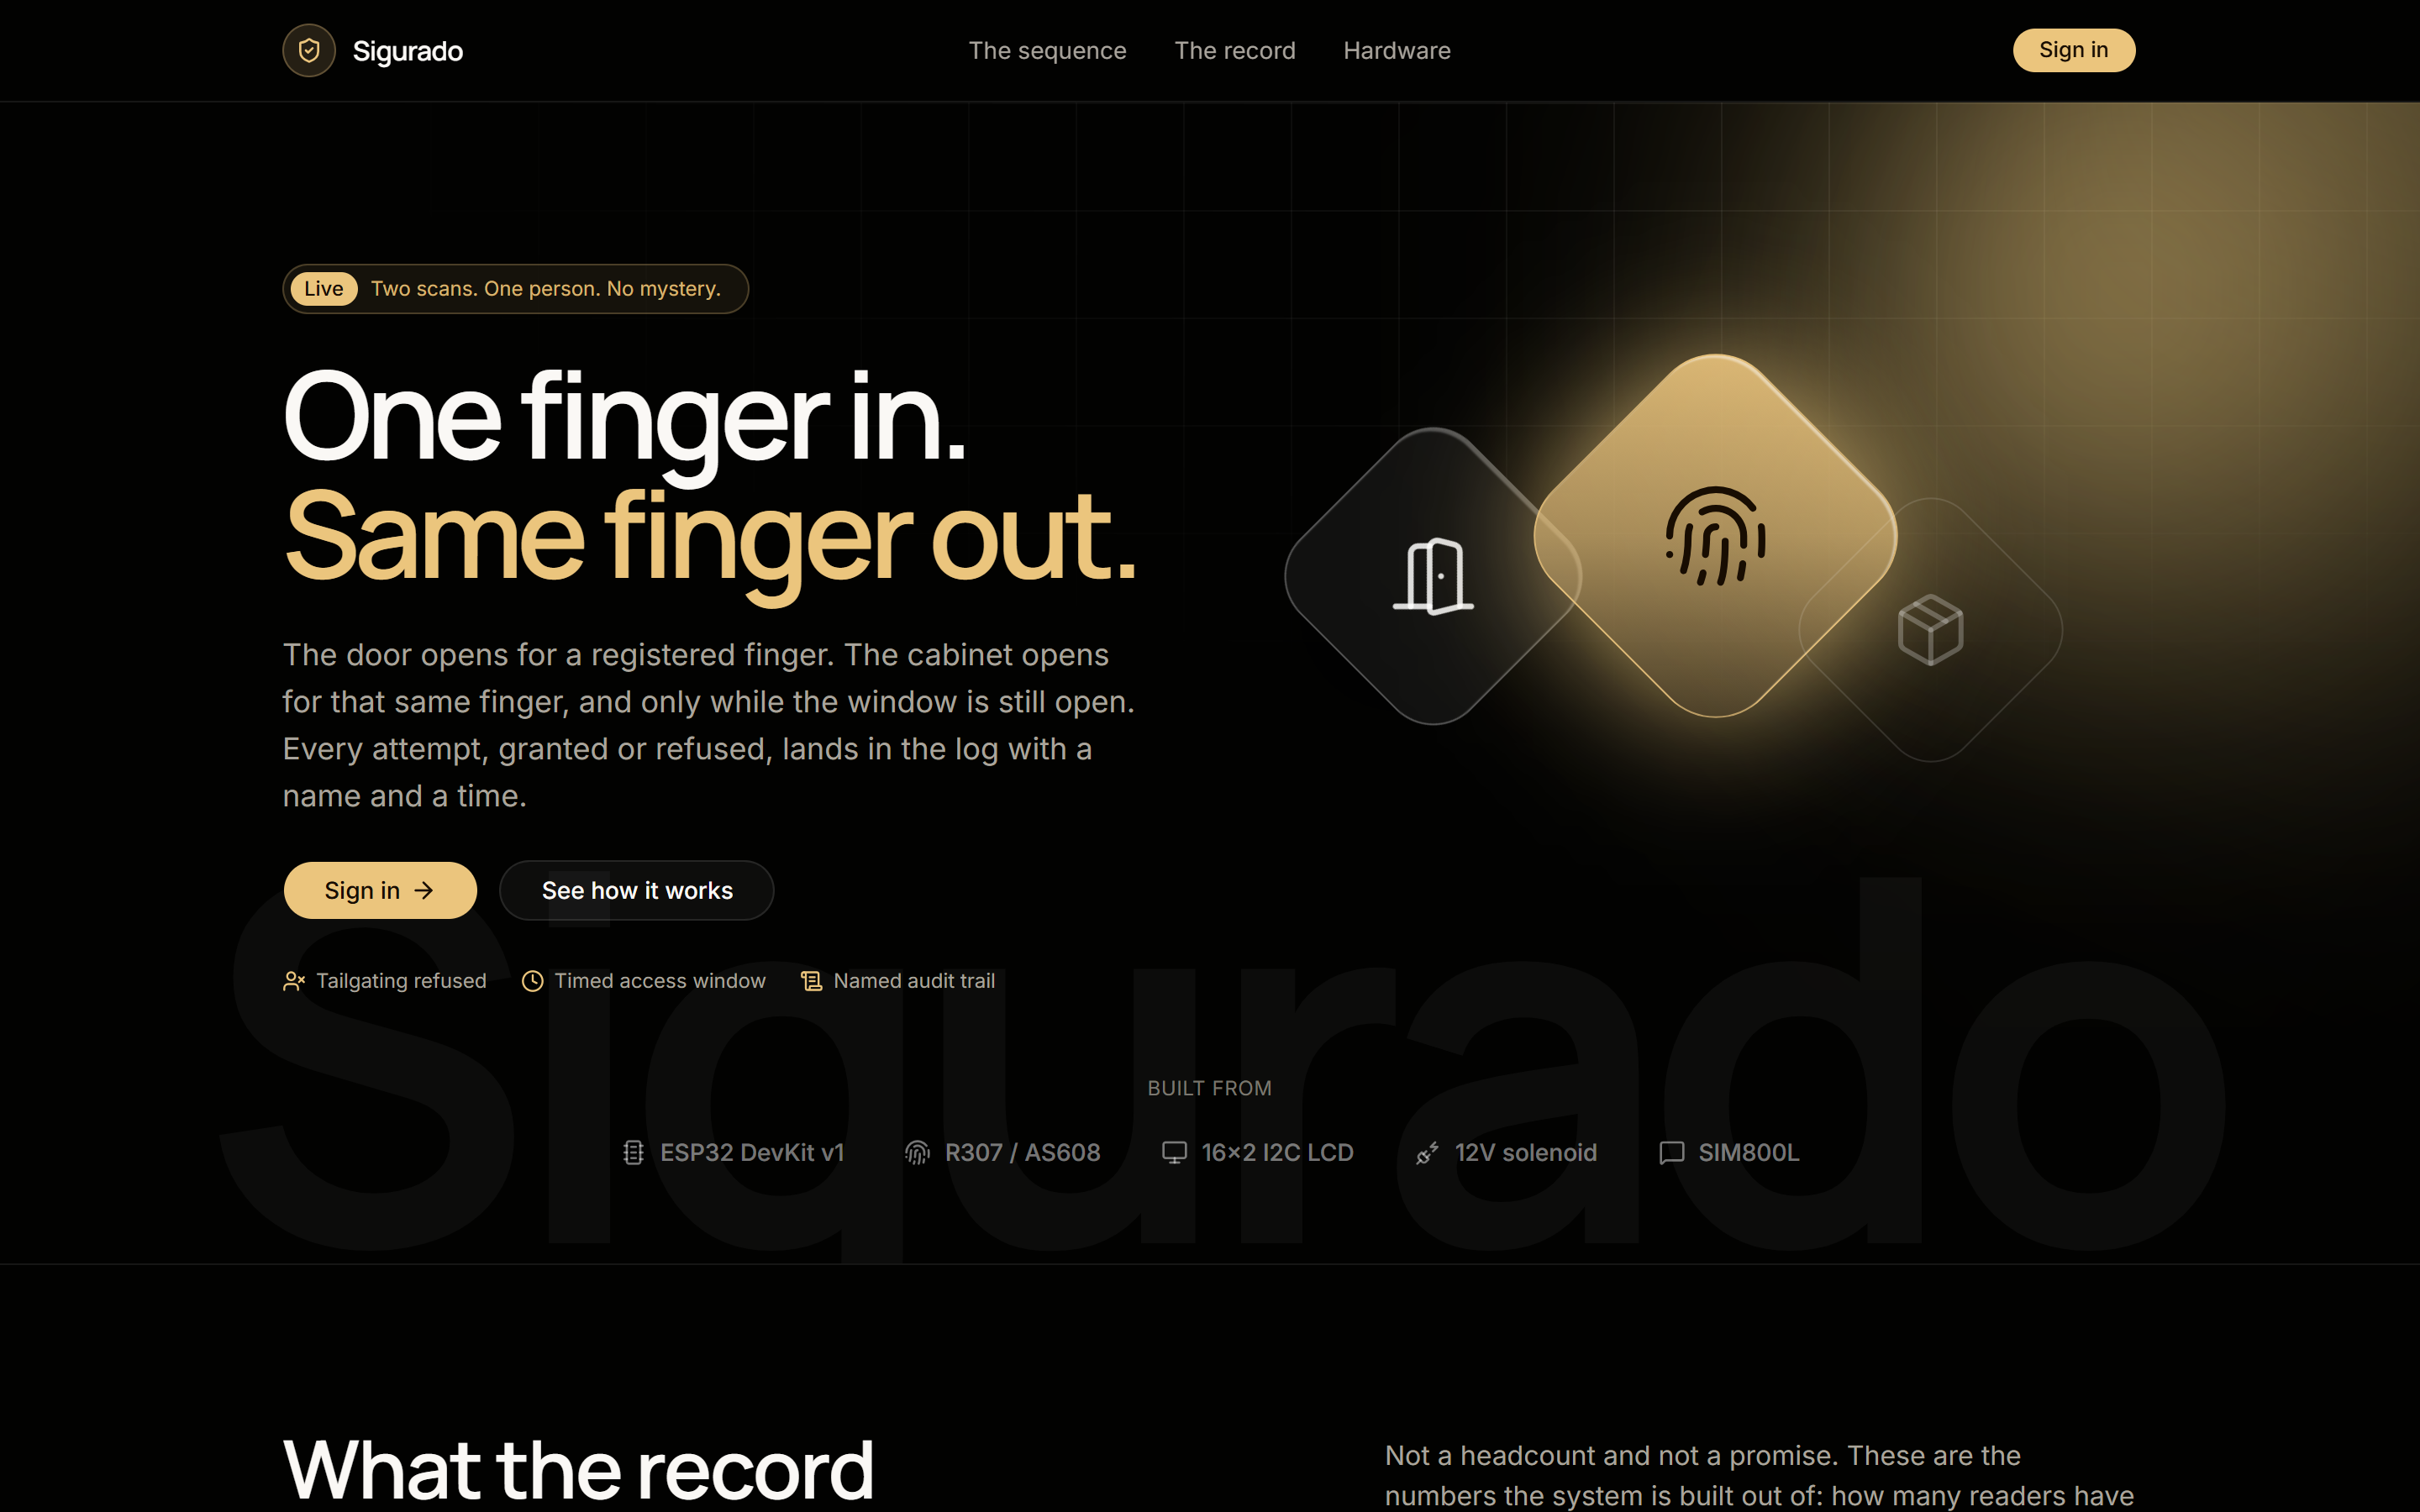
\includegraphics[width=\linewidth]{figures/web-landing.png}
\end{figure}

\subsectionhead{What Each Role Sees}

Signing in decides what the rest of the site shows. A student sees only their
own scans and their own borrowed items. A member of faculty sees everything but
can change nothing. An administrator runs the room: accounts, readers, alerts,
and the stored data. The rule the site enforces is that a student must never see
another student's record, and that nobody at all can edit a reader event.

Figure~\ref{fig:web-dashboard} shows the administrator view. The four counters
along the top answer the question a custodian actually asks on walking in: is
anyone inside the window right now, how many scans have happened today, how many
were refused, and how much was taken. Below them sit the live door sessions,
each with its own countdown, and the stream of decisions as they arrive.

The figure was captured on a quiet morning, so the counters read zero and both
panels are showing their empty state. That is deliberate rather than
unfinished. An empty panel that says only ``no data'' teaches a user nothing, so
each one instead explains what will appear there and when a session or a
decision will cause it. A custodian who has never seen the system before can
therefore read the screen on a quiet day and still understand what it will do on
a busy one.

\begin{figure}[H]
\centering
\caption{The administrator dashboard, showing live sessions and the decisions as
they arrive}
\label{fig:web-dashboard}
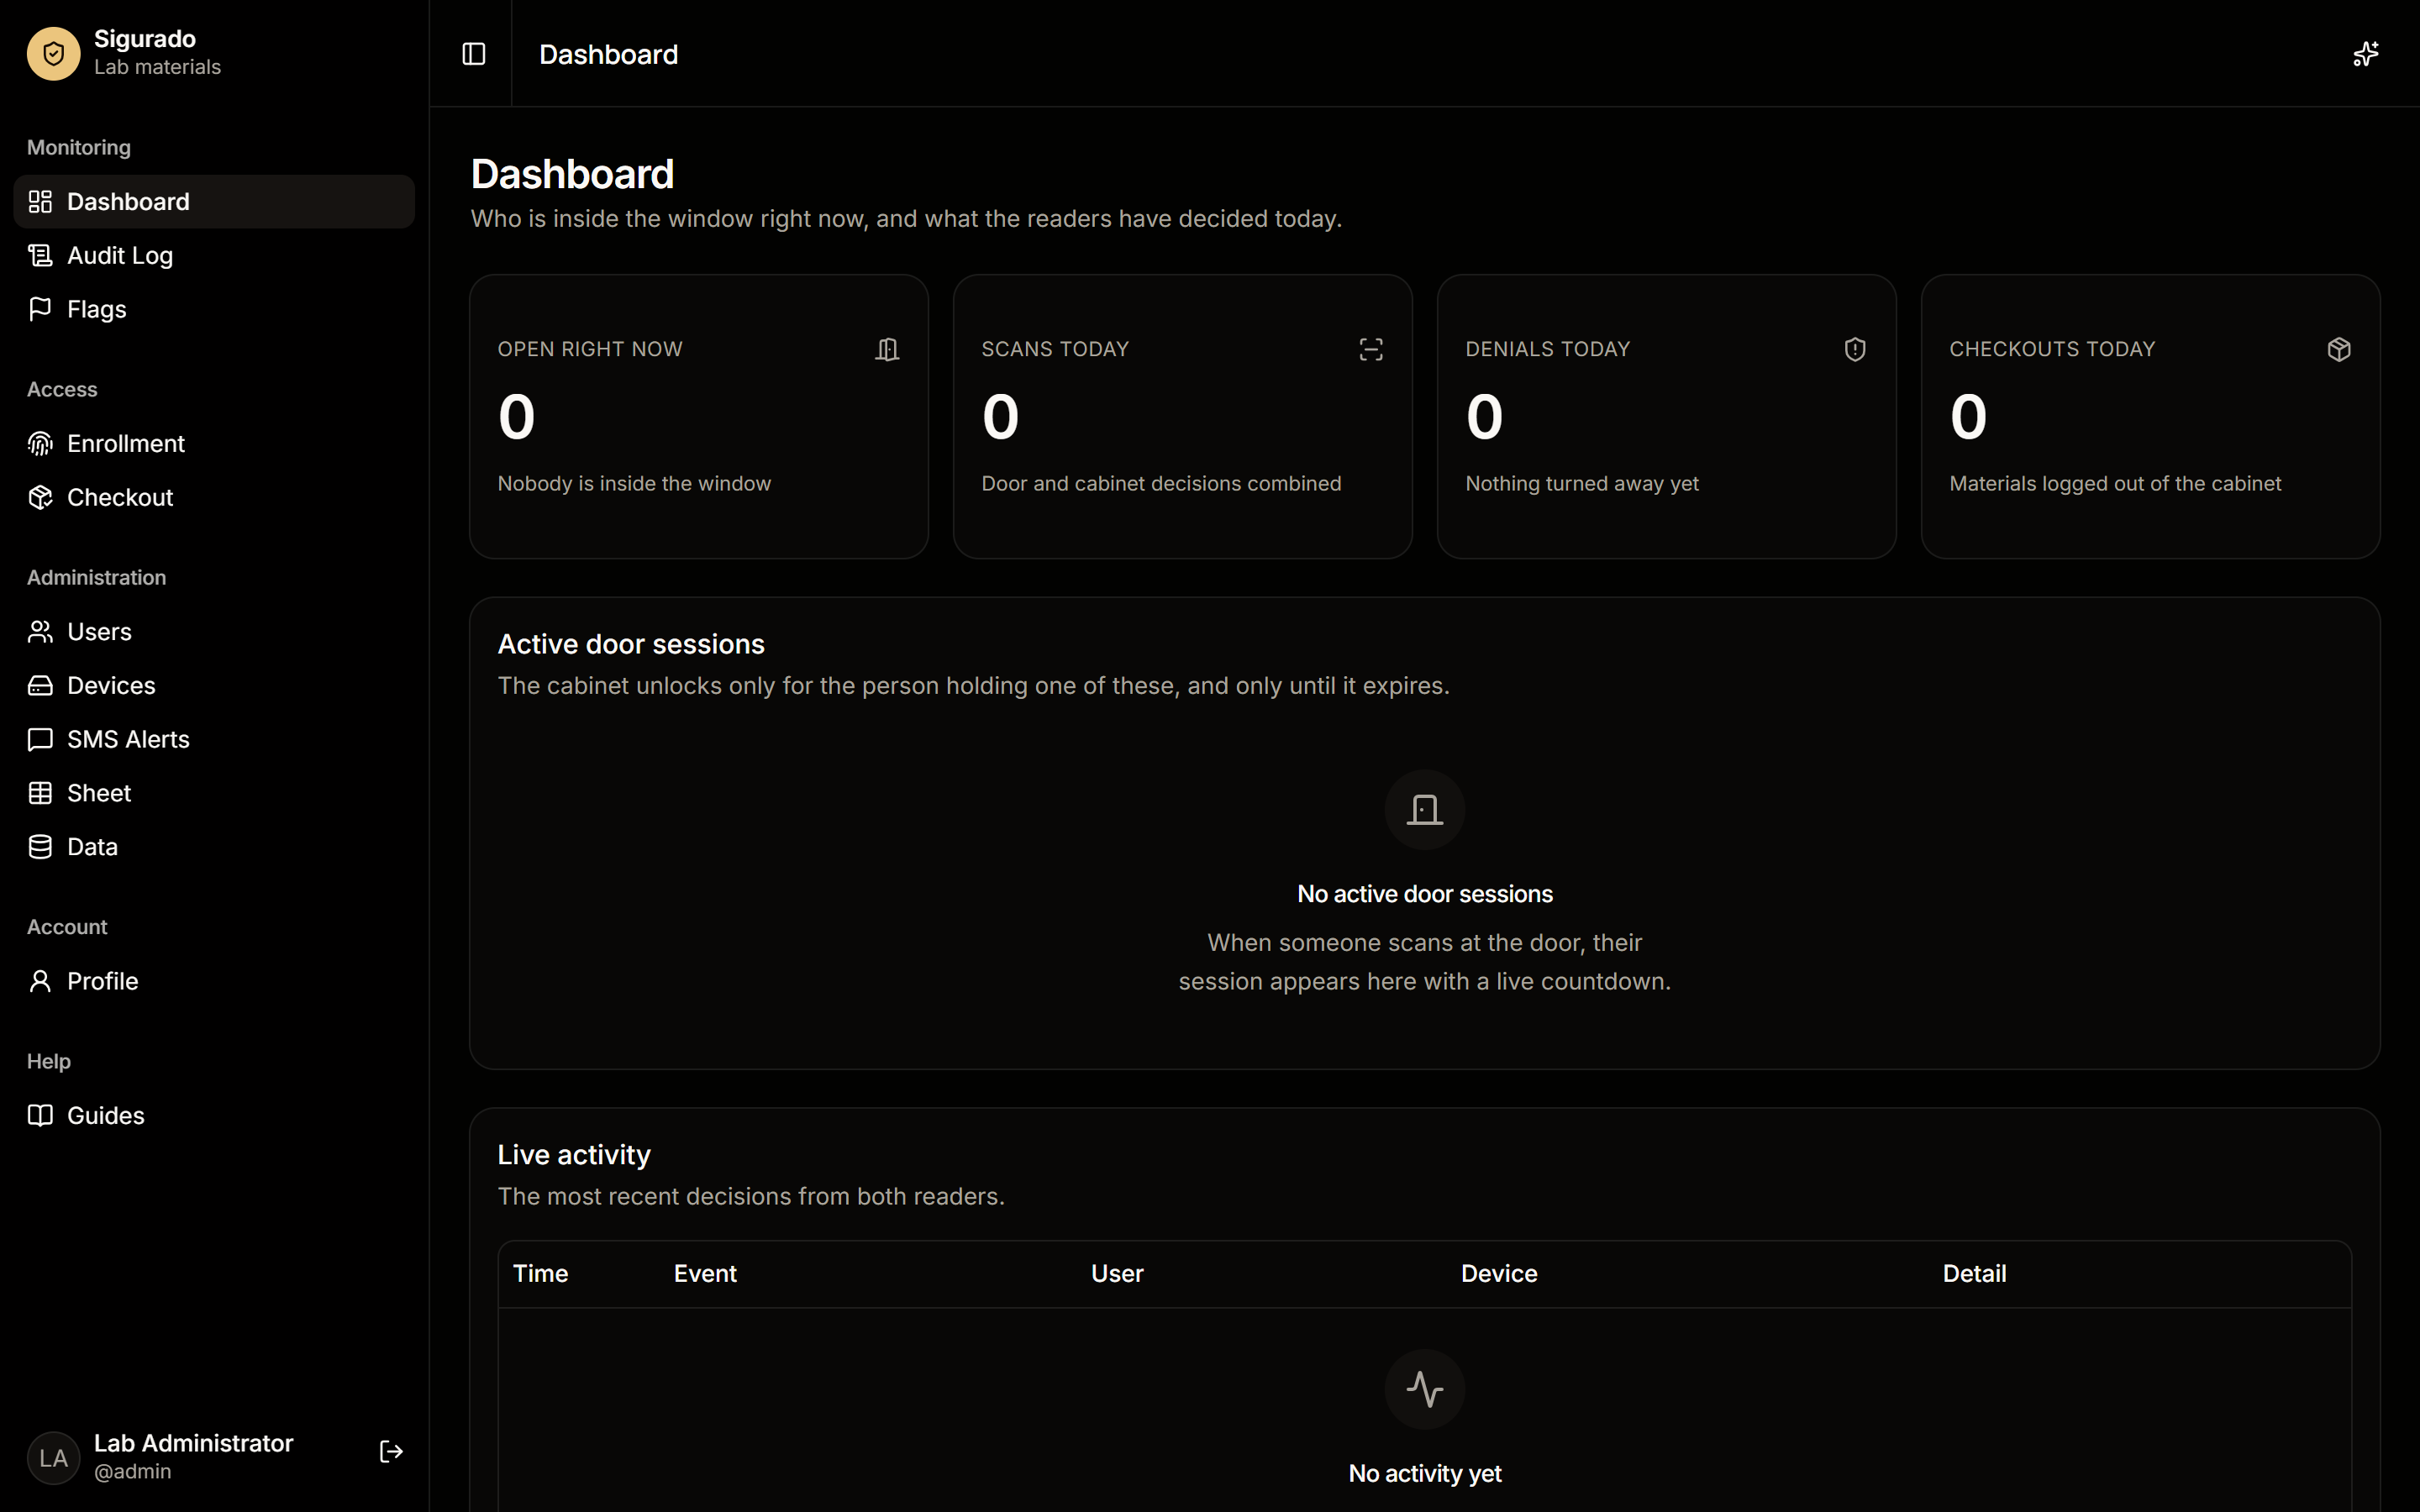
\includegraphics[width=\linewidth]{figures/web-dashboard.png}
\end{figure}

\subsectionhead{The Record}

Figure~\ref{fig:web-sheet} shows the trail as a spreadsheet. Every row is
something a reader reported: a door opened, a cabinet unlocked, a finger
refused, an enrollment code issued. Each carries the time, the person where one
is known, the finger slot, and the reader that saw it. Refusals sit in the same
list as grants, which is what makes a tailgating attempt countable rather than
invisible.

\begin{figure}[H]
\centering
\caption{The trail as a spreadsheet, with grants and refusals in the same list}
\label{fig:web-sheet}
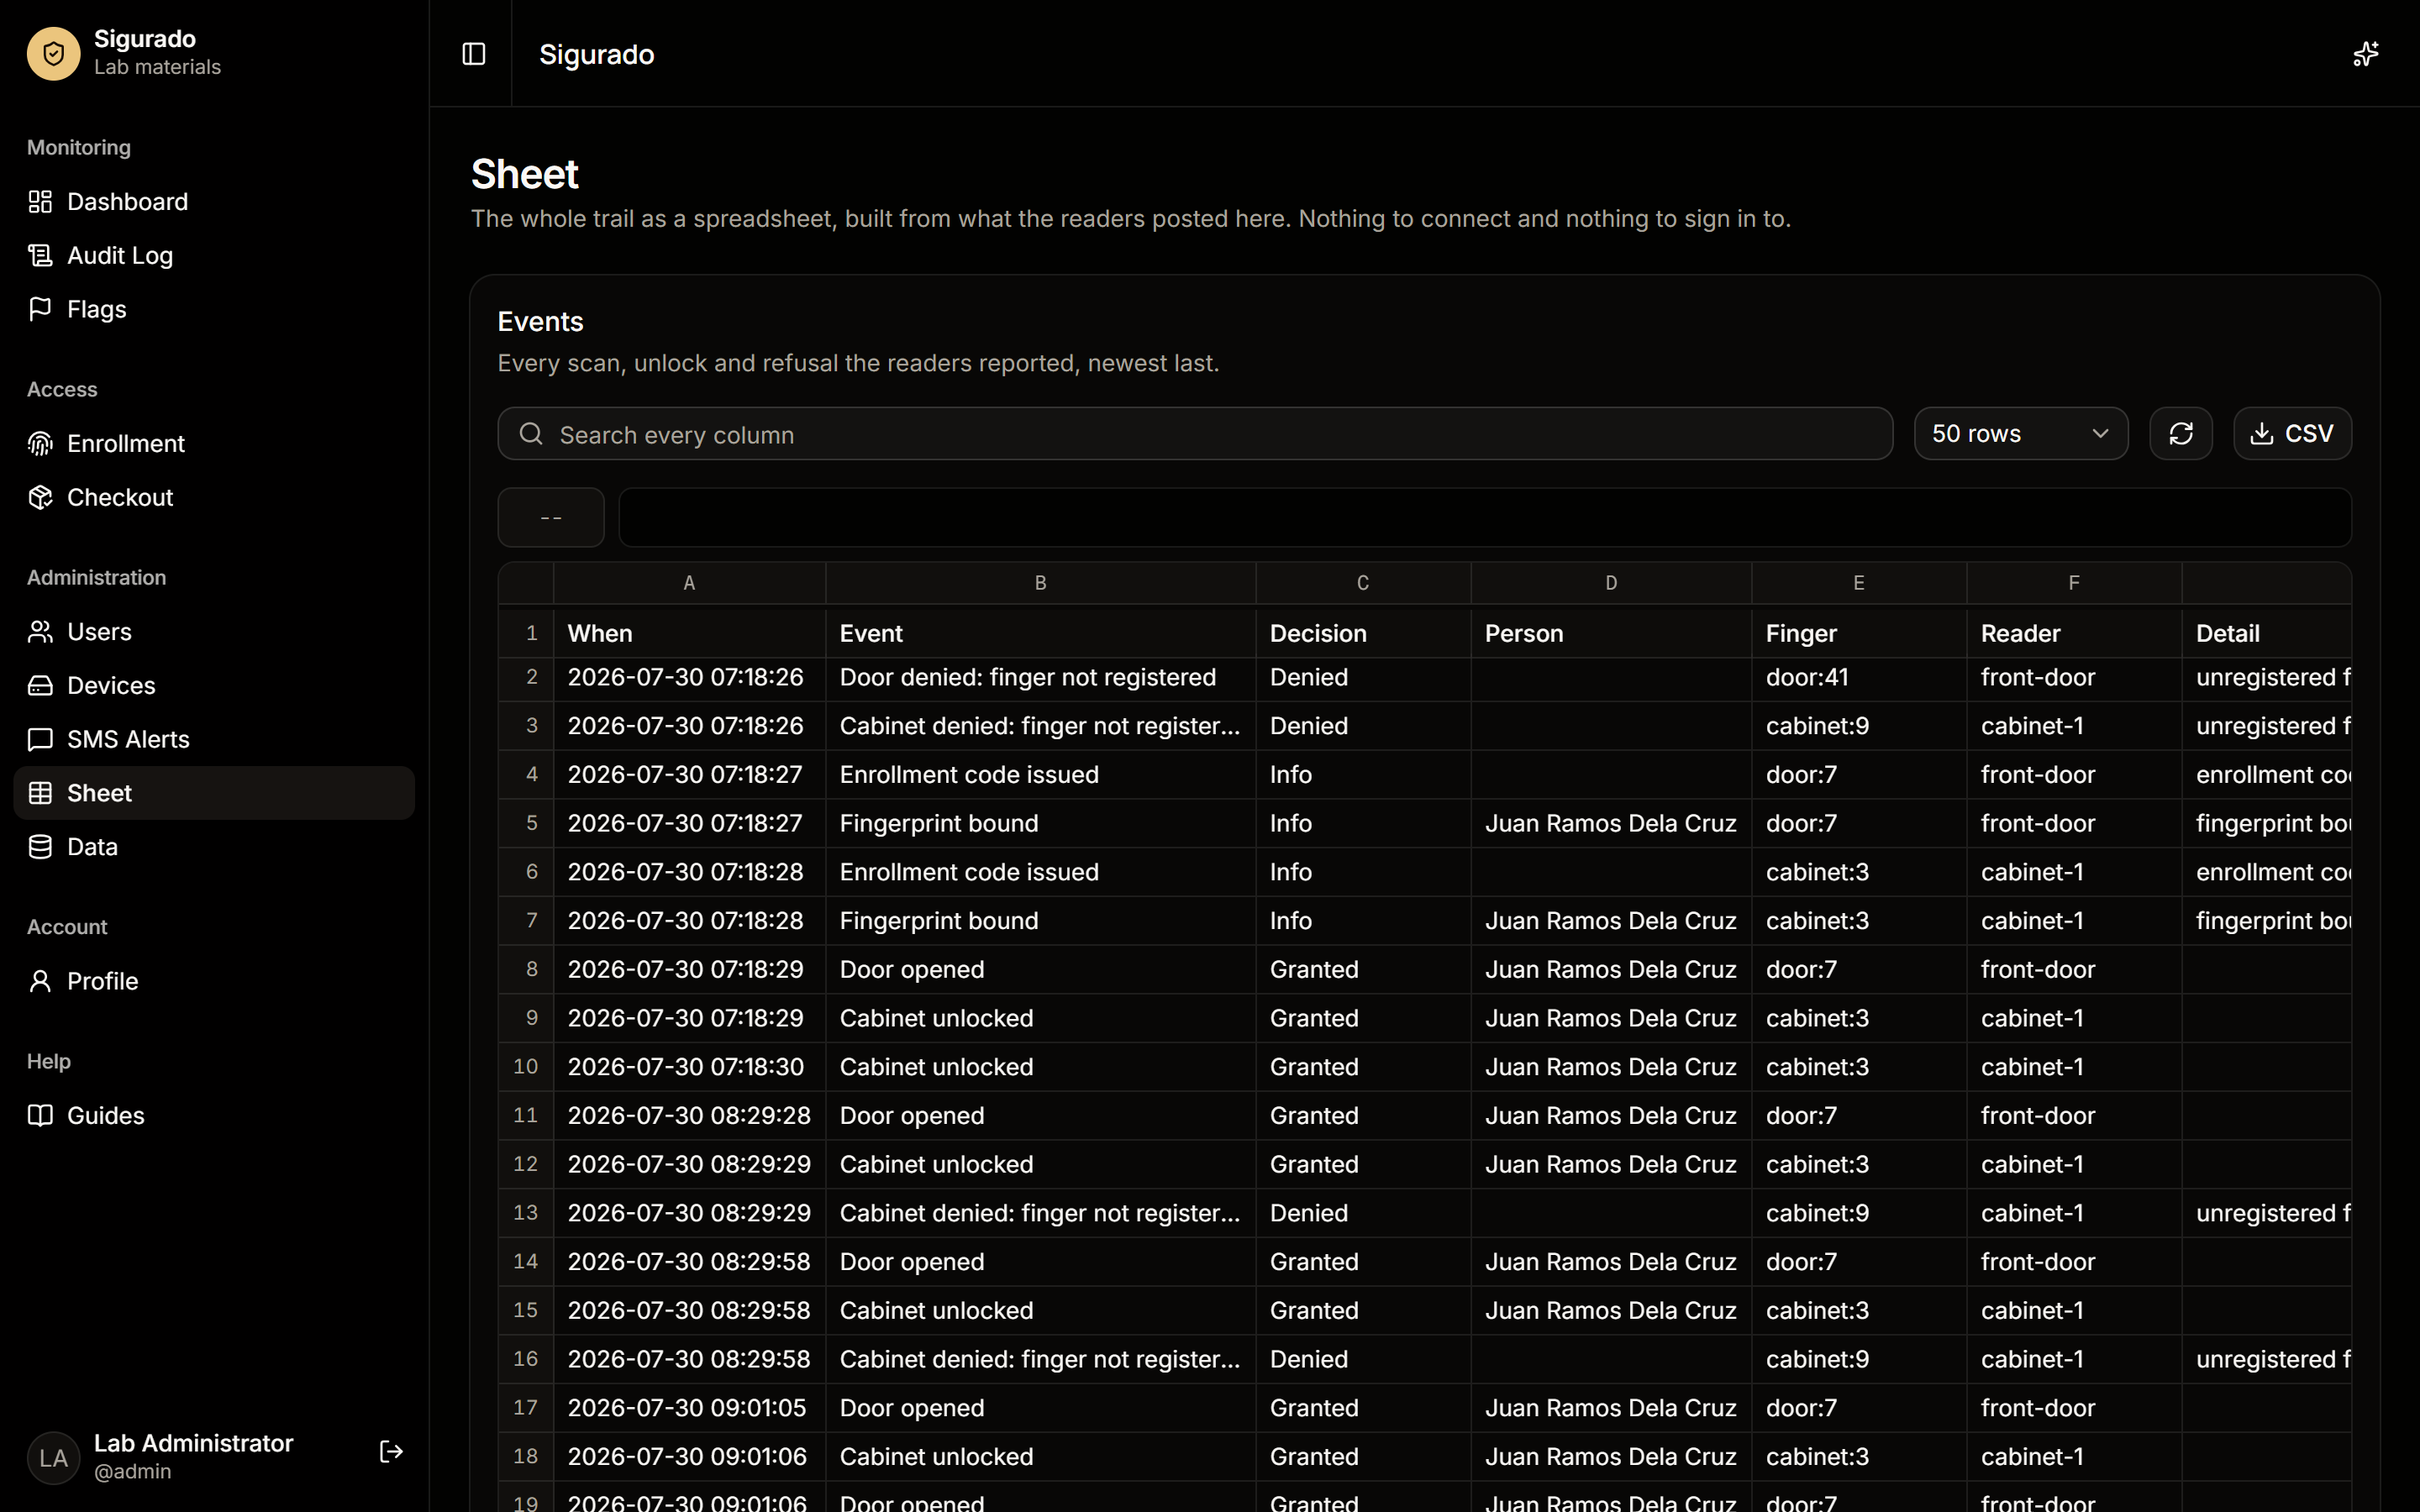
\includegraphics[width=\linewidth]{figures/web-sheet.png}
\end{figure}

The same page exports to CSV, so the record can be kept outside the system as
well. The console also runs eleven checks over the trail and lists whatever does
not add up: an opening with no borrow record behind it, a finger tried
repeatedly and refused, an opening outside laboratory hours, a reader that has
gone quiet. These are the questions a person would have to ask by hand if the
record were on paper.

\subsectionhead{On a Phone}

Most people will reach the site on a phone, standing at the cabinet with the
one-time code still on the screen in front of them. The whole console is built
to work at that size, not just to survive it.
Figure~\ref{fig:web-mobile} shows three of those screens.

\begin{figure}[H]
\centering
\caption{The site on a phone: the public page, the dashboard, and the checkout
form where the one-time code is entered}
\label{fig:web-mobile}
\begin{minipage}[t]{0.31\linewidth}
  \centering
  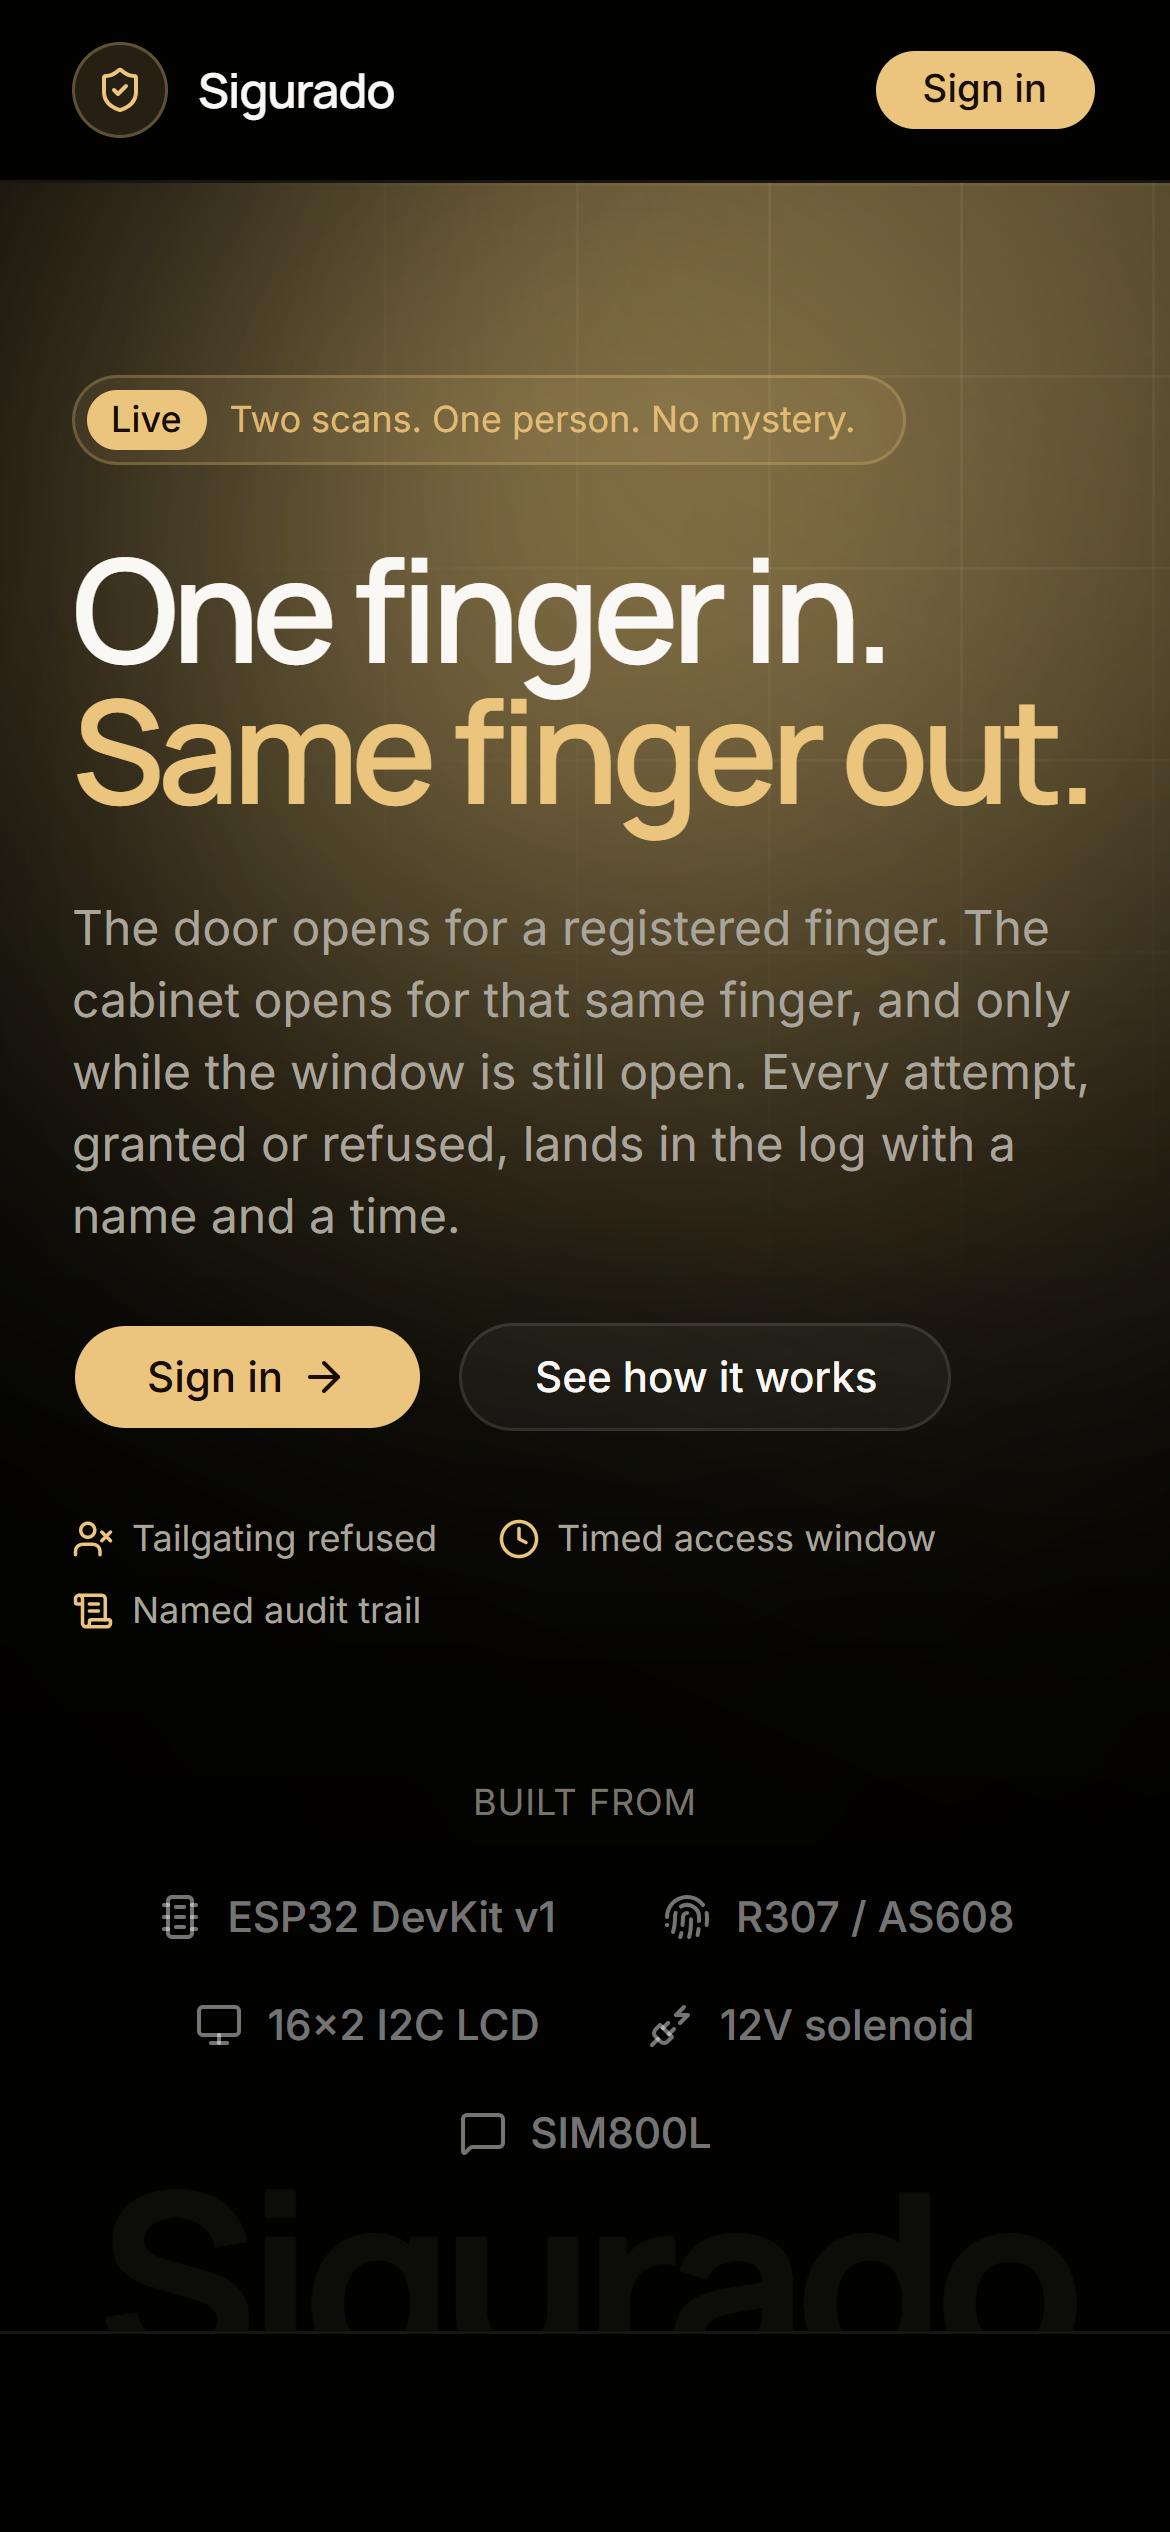
\includegraphics[width=\linewidth]{figures/mob-landing.png}
\end{minipage}\hfill
\begin{minipage}[t]{0.31\linewidth}
  \centering
  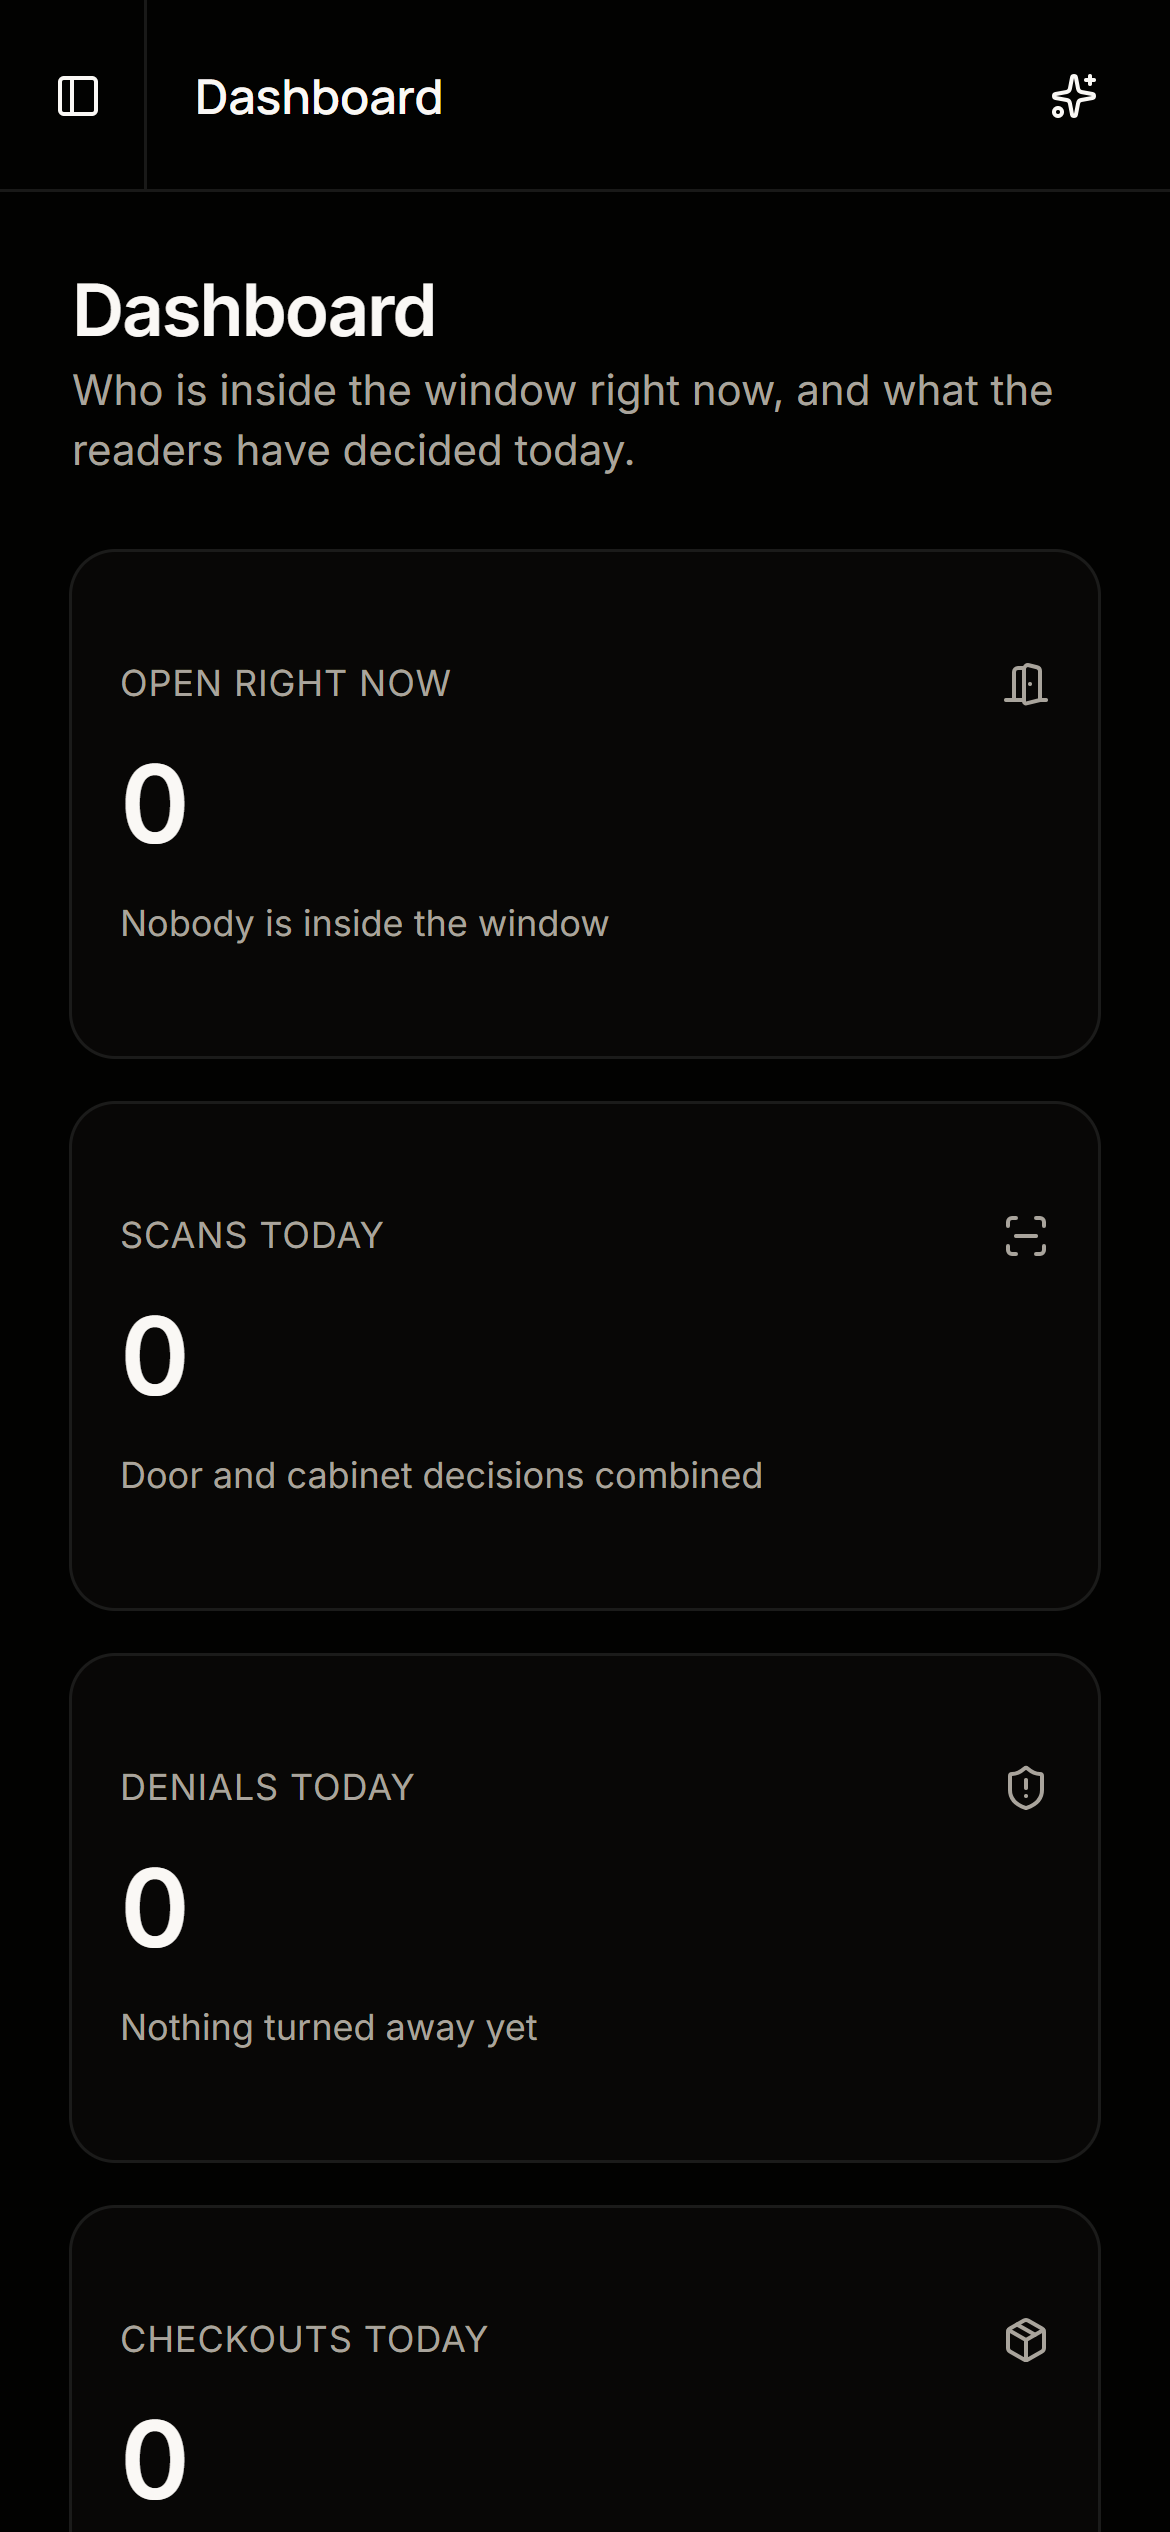
\includegraphics[width=\linewidth]{figures/mob-dashboard.png}
\end{minipage}\hfill
\begin{minipage}[t]{0.31\linewidth}
  \centering
  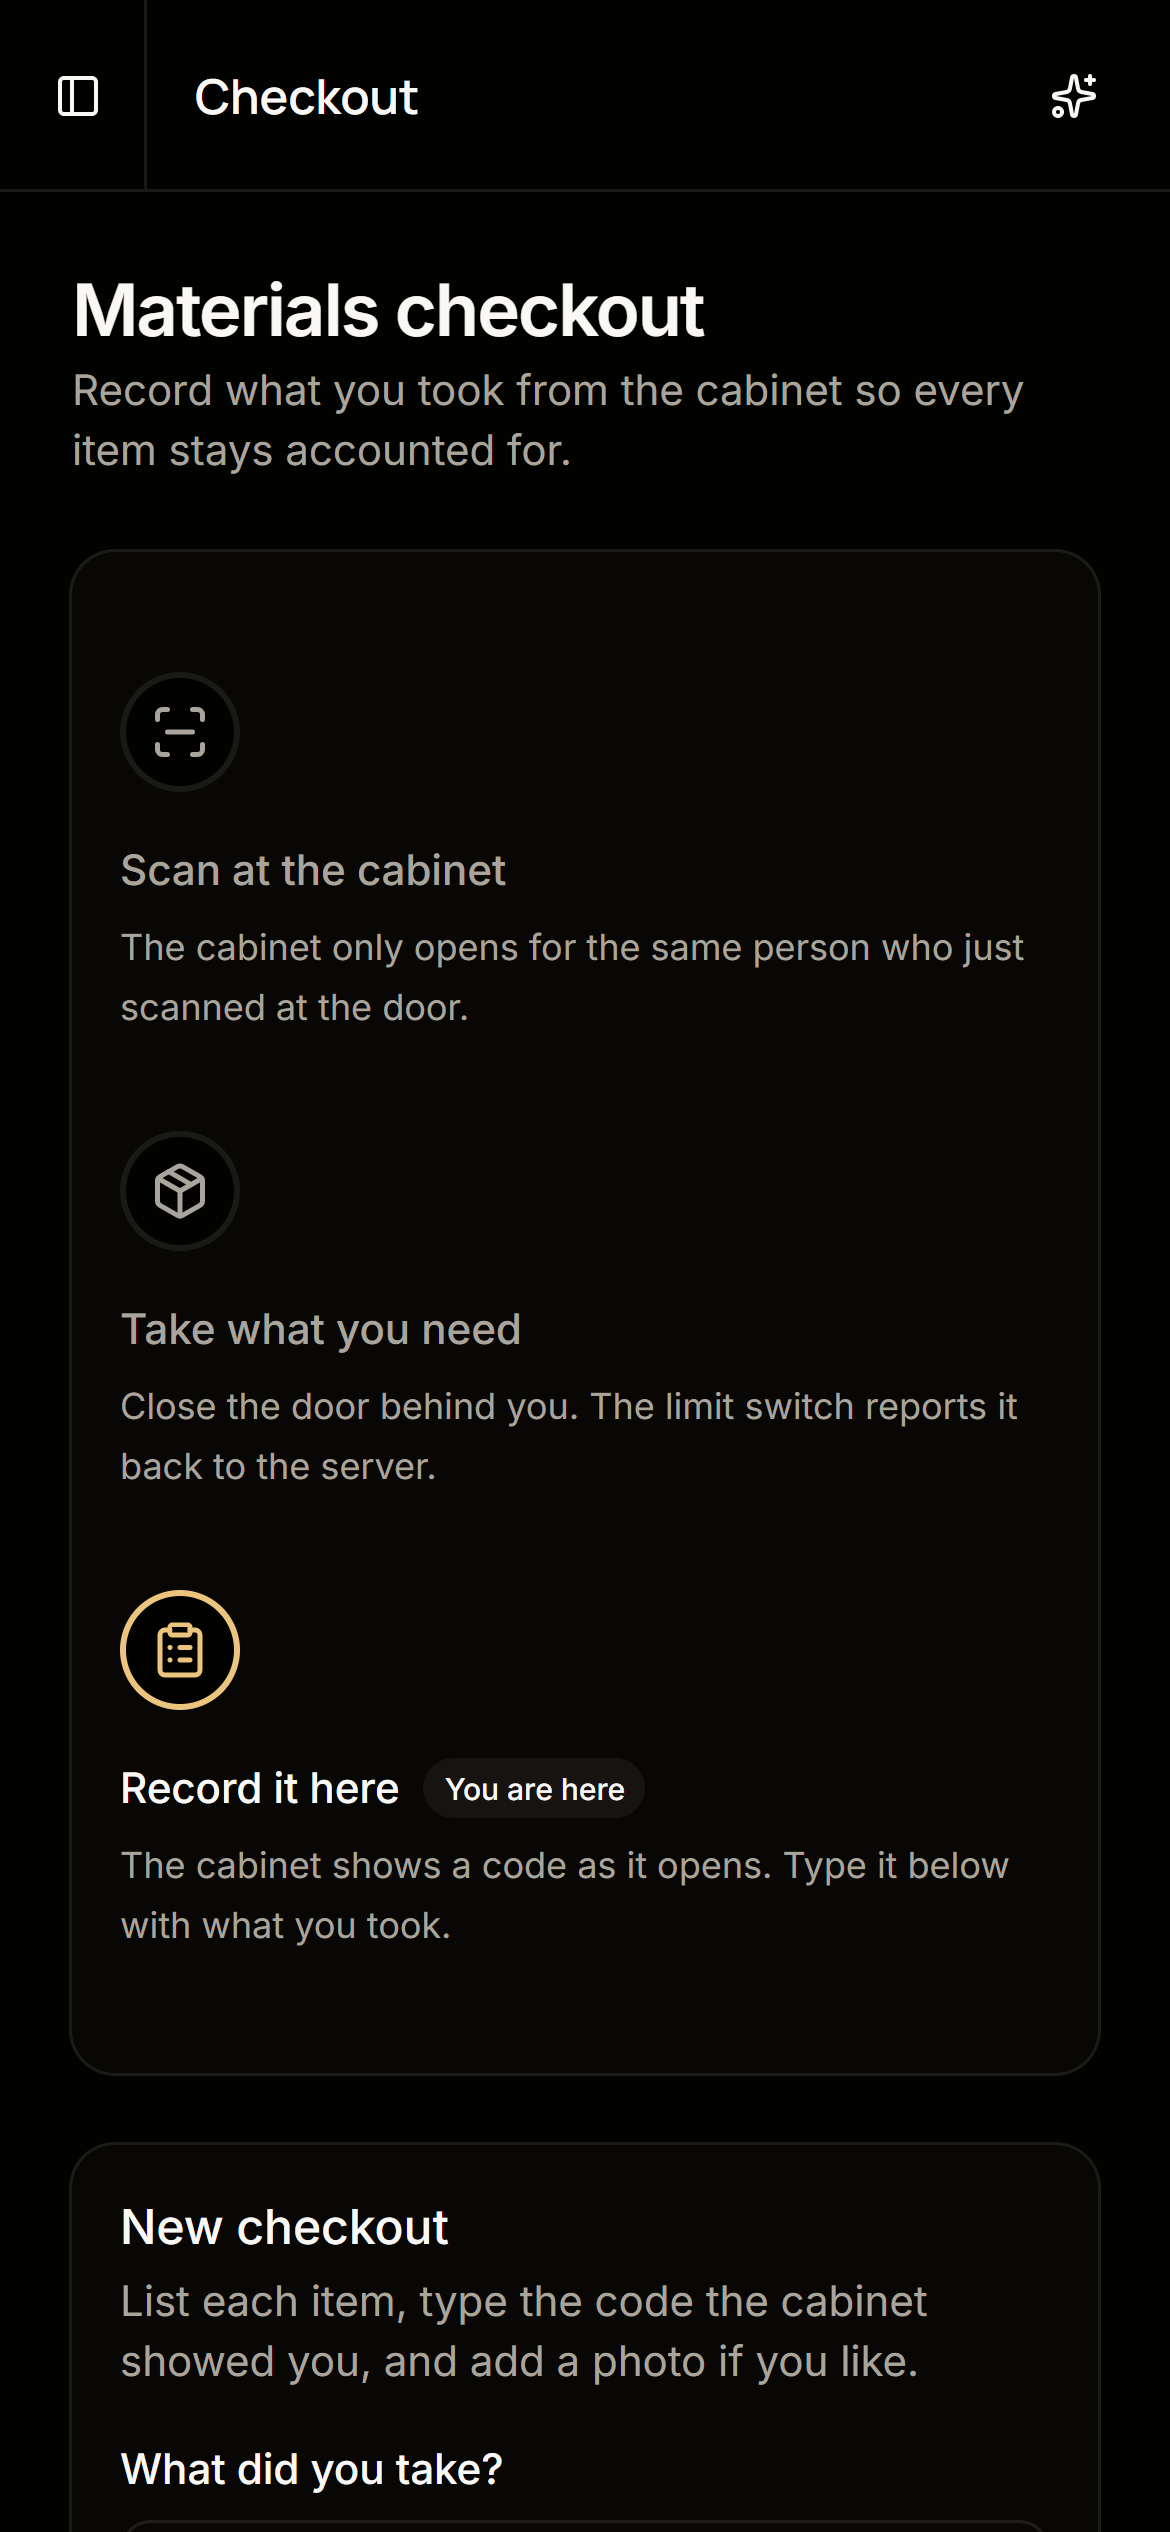
\includegraphics[width=\linewidth]{figures/mob-checkout.png}
\end{minipage}
\end{figure}

Three things change on a small screen. The side menu folds away behind a button,
so the content gets the full width. The counters stack instead of sitting in a
row. The record tables scroll sideways rather than shrinking their text, because
a column of times squeezed to four characters is worse than one the reader has
to push across.
